\section{Evaluation}
\label{sec:eval}


We evaluate our {\clsm\/} implementation versus a number of open source competitors.
%, in terms of throughput and latency, on a suite of benchmarks.
In Section~\ref{sec:microbenchmarks}, our experiments are based on  synthetic CPU-bound workloads.
In Section~\ref{sec:realworkloads} we use real web-scale application workloads.
Finally, in Section~\ref{sec:heavyCompaction}, we use a synthetic disk-bound benchmark from {\rocksdb}'s benchmarks suite~\cite{RocksDBBenchmarks}.

%Our experiments include synthetic benchmarks as well as real web-scale
%application workloads. They exercise different combinations of reads, writes, read-modify-writes,
%and snapshot scans in CPU-bound scenarios.

Our platform is a Xeon E5620 machine with 2 quad-core CPUs, each core with
two hardware threads (16 hardware threads overall).
The server has 48GB of RAM and 720GB SSD storage\footnote{Composed of four 240GB SSD SATA/300 OCZ Deneva MLC, configured as RAID-5.}.

We vary the concurrency degree in our experiments from one to sixteen worker threads performing operations;
these are run in addition to the maintenance compaction thread (or threads in Section~\ref{sec:heavyCompaction}).


We compare {\clsm} with four open-source LSM data stores: {\leveldb}~\cite{leveldb},
{\hyperleveldb}~\cite{Hyperdex2012,HyperLevelDB}, {\rocksdb}~\cite{RocksDB}, and {\blsm}~\cite{BLSM2012}.
{\hyperleveldb} and {\rocksdb} are extensions of  {\leveldb} that employ specialized  synchronization to improve parallelism
(see~\cite{RocksDBOptimizedLocks}),
and {\blsm\/} is a single-writer prototype that capitalizes on careful scheduling
of merges.
%
Unless stated otherwise, each LSM store is configured to employ an in-memory
component of 128MB \eurosys{E2}{(this is the standard value in key-value stores
like HBase)}; we use the default values of all other configurable parameters.

Recall that in LSM-DS, component merges occur as a background process, which is often called \emph{compaction}.
All systems except {\rocksdb} use a single background thread for compaction.
{\rocksdb} has a configurable parameter determining the maximum number of compaction threads,
which we set to one\footnote{This is the default value in {\rocksdb}.}, except in Section~\ref{sec:heavyCompaction}.
We note that in experiments that involve writes (i.e., put operations), the compaction thread is working a significant  portion of the time --- in the CPU-bound experiments reported in Sections~\ref{sec:microbenchmarks} and~\ref{sec:realworkloads}, we found that it runs  roughly between a quarter and three-quarters of the time, in all systems. In Section~\ref{sec:heavyCompaction} we consider disk-bound workloads, where compaction runs virtually all the time, and creates a bottleneck.

\subsection{Synthetic Workloads}
\label{sec:microbenchmarks}


We start with a set of benchmarks that exercise the systems in a variety of controlled settings.
%The benchmarks experiment with concurrency degrees from 1 to 16 threads.
Our experiment harnesses a 150GB dataset (100x the size of the
collection used to compare {\hyperleveldb\/} to {\leveldb\/} in the publicly available
benchmark~\cite{hyperdex}).
The key-value pairs have 8-byte keys, and the value size is $256$ bytes.


 {\bf {Write performance.}}
We start by exploring a write-only workload.
The keys are drawn uniformly at random from the entire range.
(Different distributions lead to similar results --
recall that the write performance in LSM stores is locality-insensitive.)

Figure~\ref{fig:100w_throughput} depicts the results in terms of throughput.
{\leveldb}, {\hyperleveldb\/}, and {\clsm\/} start from approximately the same point, but
they behave differently as we increase the number of threads.
{\leveldb}, {\blsm} and {\rocksdb} are bounded by their single-writer
architectures, and do not scale at all. \eurosys{E5}{Moreover, having multiple
threads contending for a single synchronization point (e.g., a writers queue)
causes the throughput to decrease.} {\hyperleveldb} achieves a $33\%$ throughput
gain with $4$ workers, and deteriorates beyond that point.
{\clsm\/}'s throughput scales $2.5$x and becomes saturated at $8$ threads. \eurosys{E4}{The degragation in write performance can be explained by cross-chip latency and cache invalidations, since only the 16 threads experiment spans more than one chip.} {\clsm\/}'s peak rate
exceeds $430$K writes/sec, in contrast with $240$K for {\hyperleveldb}, $160$K for {\leveldb} and $65$K for {\rocksdb}.
%
%Note that {\clsm\/}'s peak performance is achieved with $8$ threads. This happens due to
%intensive cache synchronization between the two CPU's, as all cores perform frequent atomic
%hardware instructions.


%\clsm's advantage can be explained via its improved CPU utilization. For example, with 8 threads {\clsm}'s per-core
%sustained utilization reaches 94\%, whereas {\leveldb}'s is just above 40\%.


Figure~\ref{fig:100w_latencyVSthroughput} refines the results by
presenting the throughput-latency perspective, where the latency is computed
for the $90$-th percentile; other percentiles exhibit similar trends.
For better readability we delineate improvement trends and omit points
exhibiting decreasing throughput. This figure marks the point in which
each implementation saturates, namely, either achieves a slight
throughput gain while increasing the latency by a factor of $2$x-$3$x or
achieves no gain at all. \eurosys{E}{It is clear that {\clsm} scales better than all competitors.}

%Figure~\ref{fig:100w_latency} compares the systems in terms of latency (the median,
%the 90\% and the 99\%), for $8$ threads.
%{\clsm} achieves the lowest latency, e.g., with
%8 threads its median write latency is 15 {\microsec}, and the 90th percentile is
%31 {\microsec}. The single-writer implementations are most vulnerable to latency
%variability -- e.g., for {\leveldb\/} and {\blsm\/} the median latencies exceed
%75 {\microsec} and 100 {\microsec}, respectively.

%{\color{red}
%Our measurements show that scans support in {\clsm}'s writes (active set
%maintenance, see Section~\ref{sec:algorithm}) incurs insignificant overhead in
%most cases.
%For applications that do not require snapshot scans, stripping the
%snapshot-support code can boost throughput in some settings up to 15\% beyond
%the demonstrated numbers.
%}



\begin{figure*}%[t]
  \centering
  \begin{subfigure}[t]{0.49\textwidth}
   \center
   \fbox{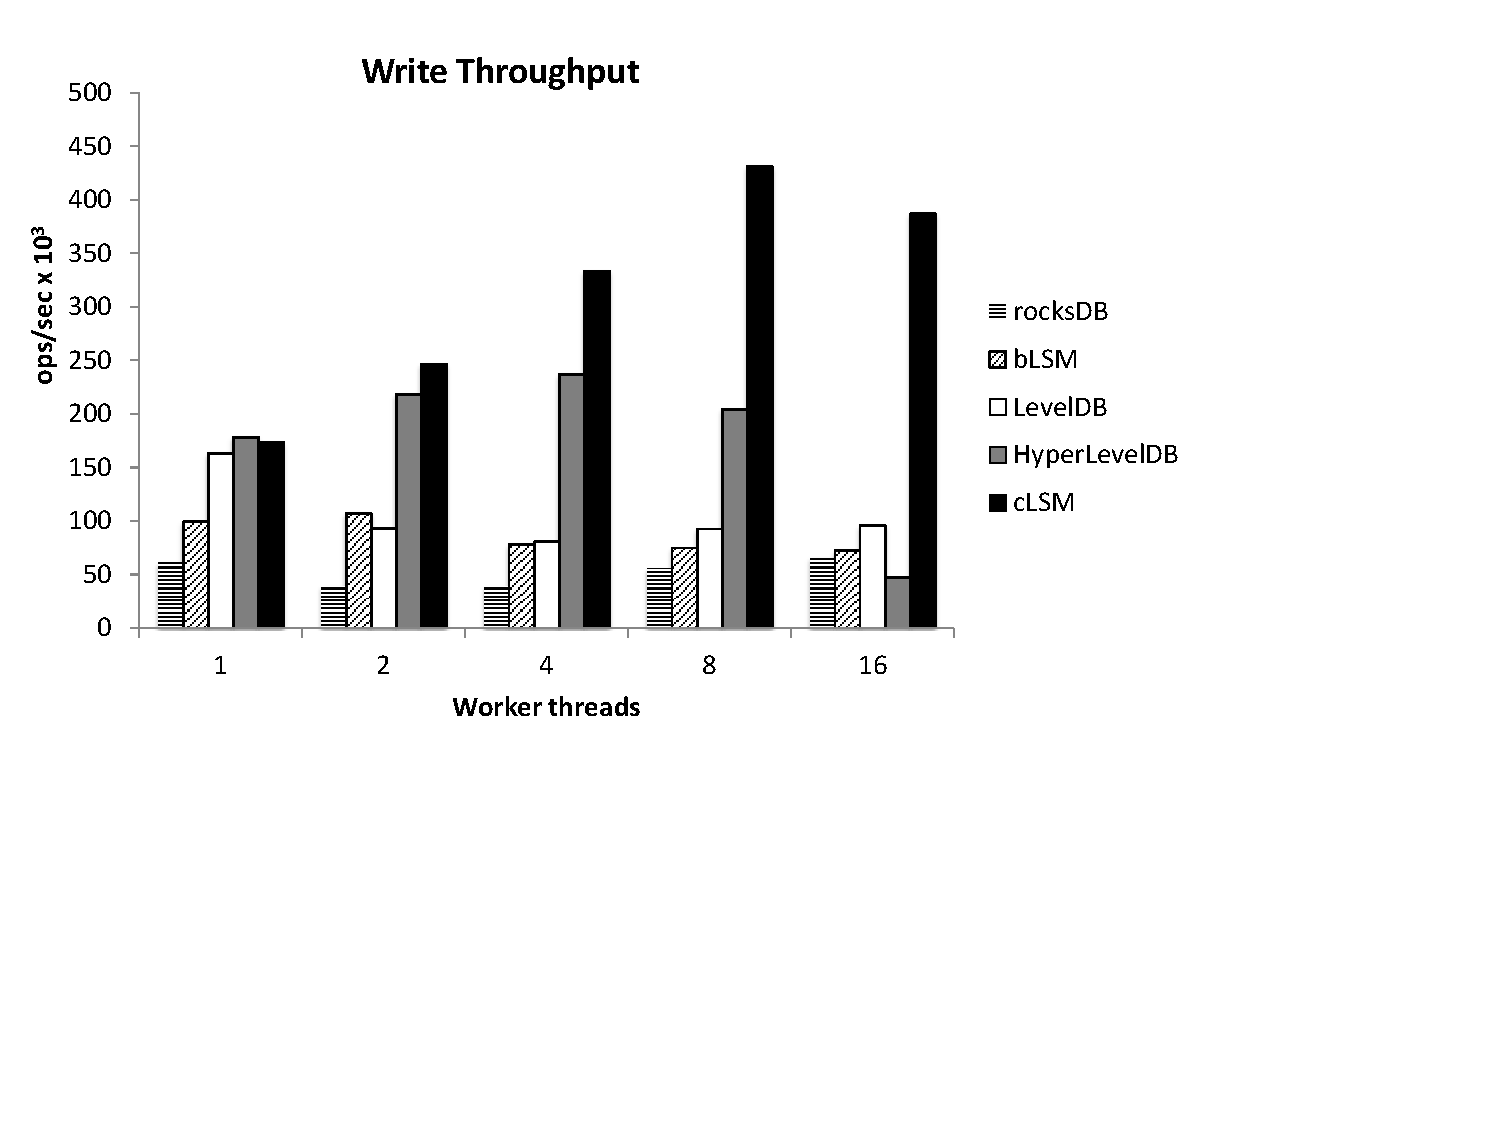
\includegraphics[width=0.9\textwidth,clip, trim =0 180 150 0]{Figures/100_write_throughput.pdf}}
		%{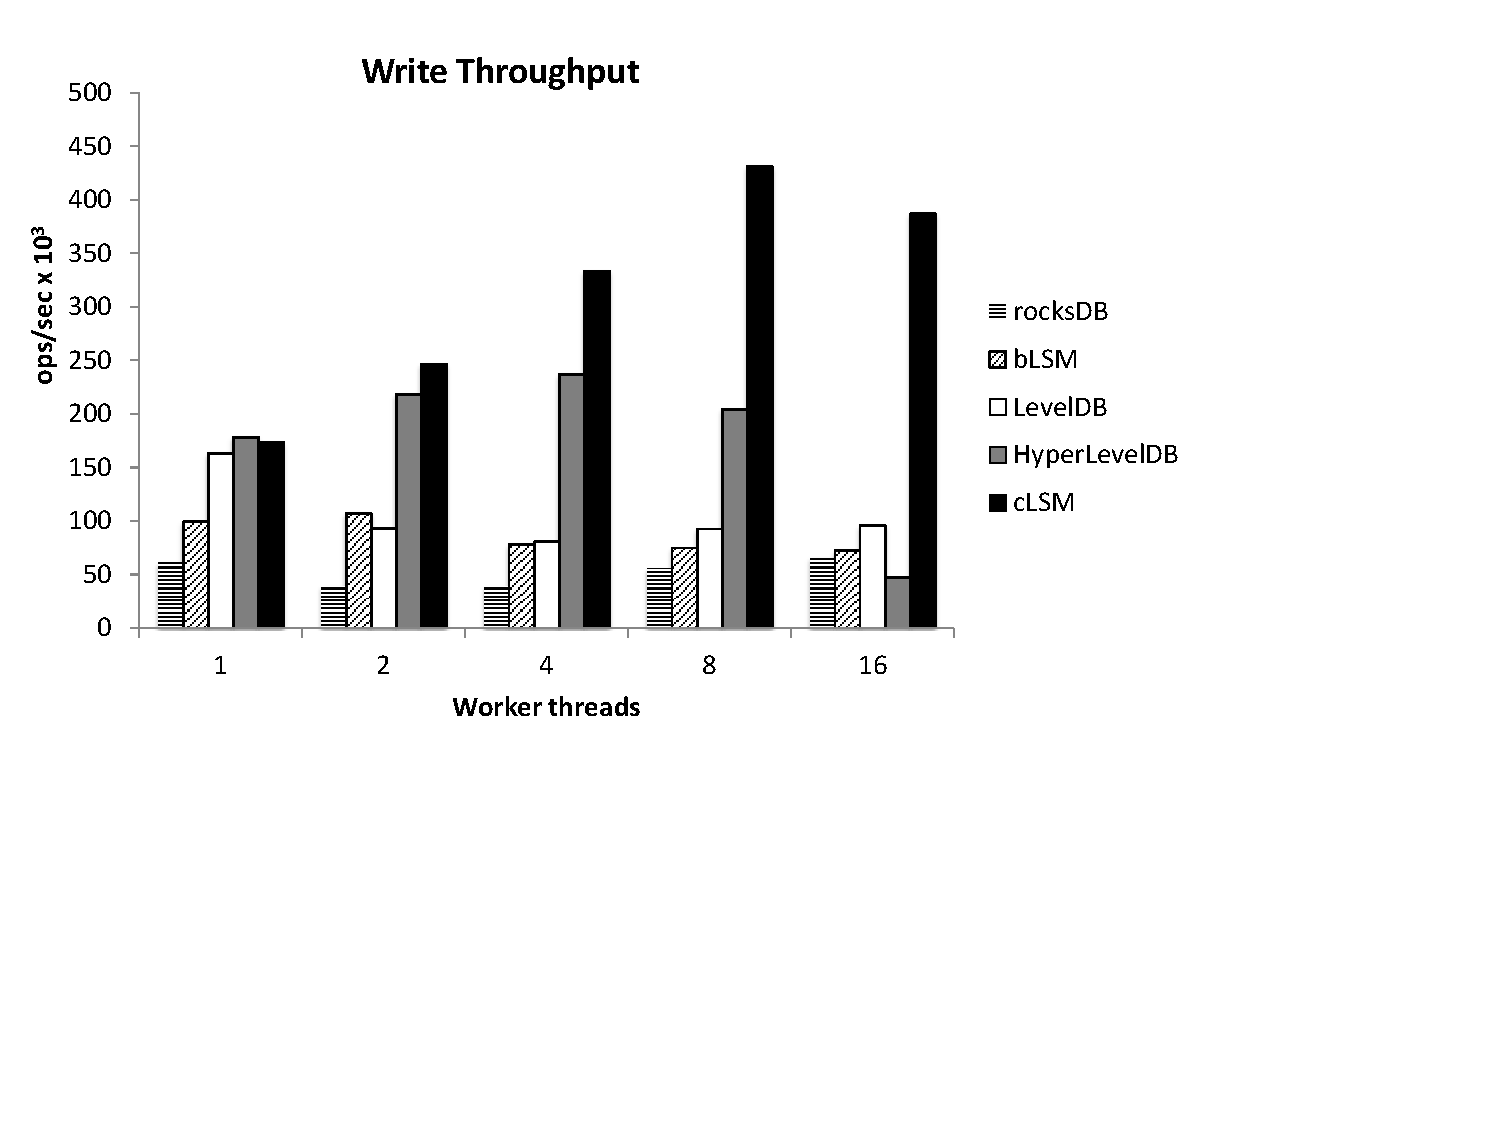
\includegraphics[height=1.8in]{Figures/100_write_throughput.pdf}}
		\caption{Throughput}
               \label{fig:100w_throughput}
  \end{subfigure}%
 %\hspace{0.2\textwidth}
  \begin{subfigure}[t]{0.49\textwidth}
   \center
		\fbox{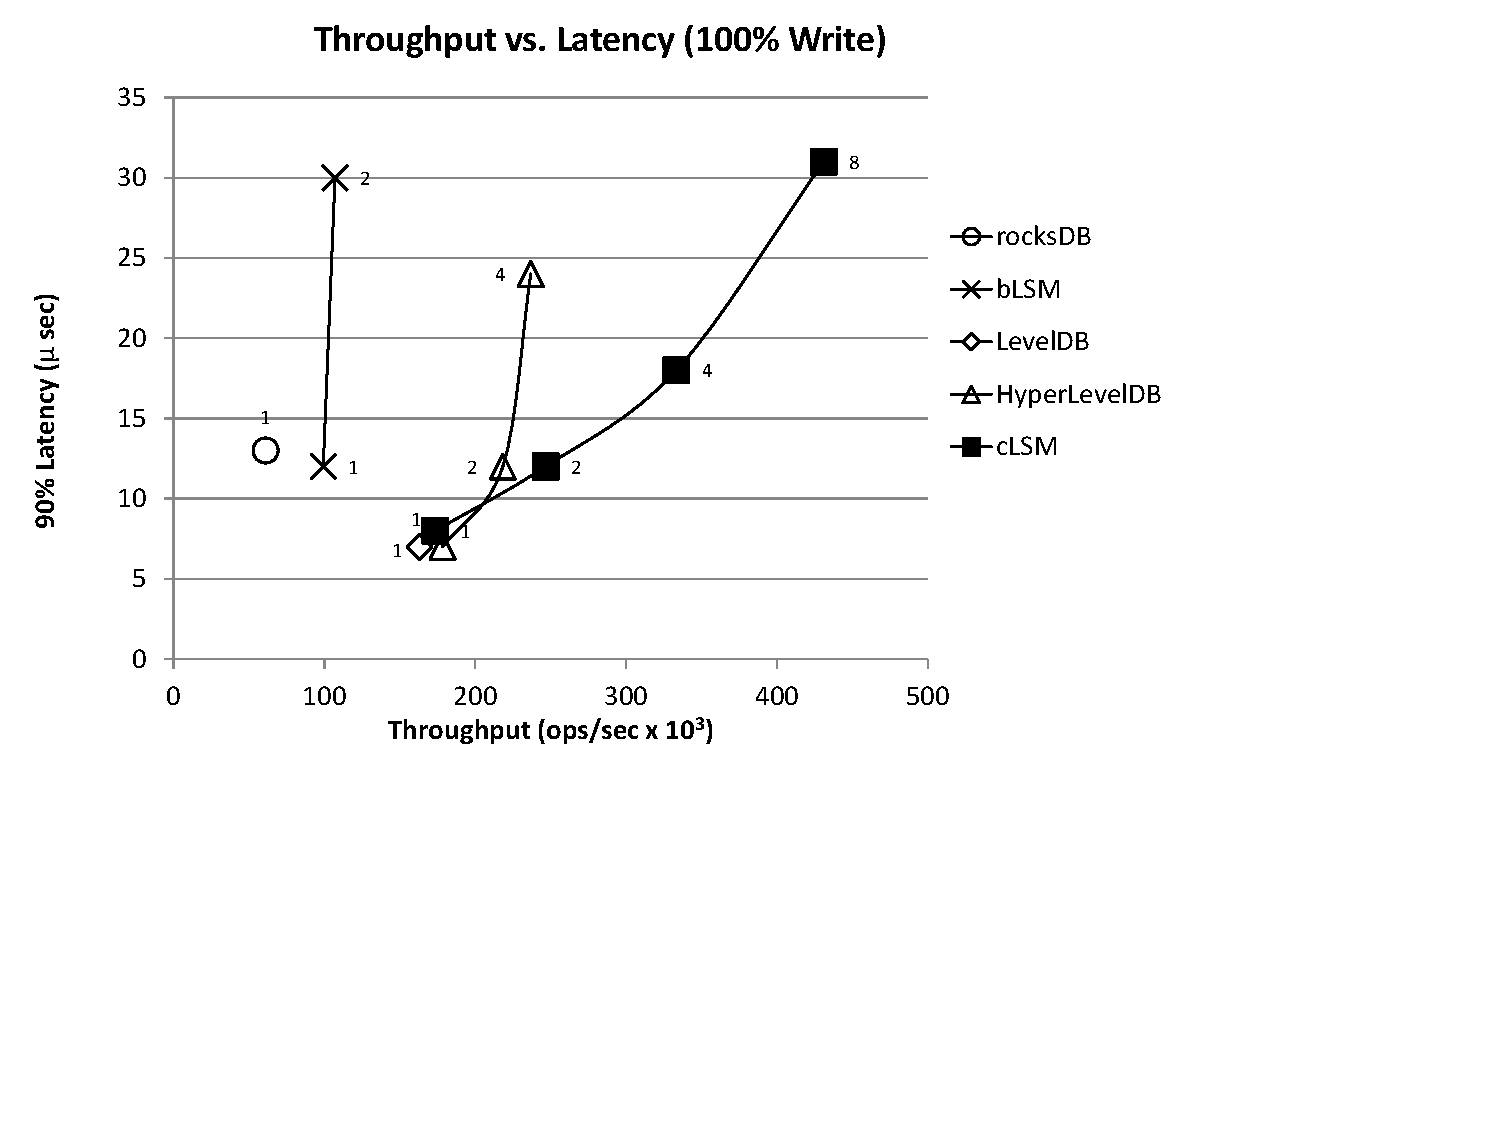
\includegraphics[width=0.9\textwidth,clip, trim =0 180 160 0]{Figures/100_write_latency_vs_throughput.pdf}}
		\caption{Throughput versus latency; each data point is labeled with the number of threads}
               \label{fig:100w_latencyVSthroughput}
  \end{subfigure}%
\caption{\bf{Write performance -- a 100\% write scenario, with the keys uniformly distributed across the domain.
{\clsm\/} scales to 8 threads and achieves 80\% throughput advantage over the closest competitor, which only scales to 4.
%With 8 threads -- {\clsm\/} is significantly faster in all latency percentiles.
}}
\label{fig:100w}
\end{figure*}





{\bf{Read performance.}}
We turn to evaluate performance in a read-only scenario. In this context,
uniformly distributed reads would not be indicative, since the system would spend most of the time in disk seeks,
devoiding the concurrency control optimizations of any meaning. Hence, we employ a skewed distribution that
generates a CPU-intensive workload: $90\%$ of the keys are selected randomly from ``popular'' blocks that
comprise $10\%$ of the database. The rest are drawn u.a.r. from the whole range. This workload is both dispersed
and amenable to caching. Its locality is similar to that of production workloads analyzed in
Section~\ref{sec:realworkloads}. All the following experiments exercise this distribution.


Figure~\ref{fig:100r_throughput} demonstrates throughput scalability.
{\leveldb\/} and  {\hyperleveldb\/} exhibit similar performance.
Neither scales beyond $8$ threads, reflecting the limitations of {\leveldb}'s concurrency control, \eurosys{E4}{namely, read operations blocking even when data is available in memory.}
On the other hand, {\clsm} and {\rocksdb} scale all the way to $128$ threads, far beyond
the hardware parallelism
(more threads than cores are utilized, since some threads block when reading data from disk).
In all cases, {\rocksdb} is not only slower than \eurosys{E}{{\clsm}, but even slower than {\leveldb\/}}.
%{\blsm} has similar performance in all cases.
In this experiment, the peak throughput of {\clsm} is almost $1.8$ million
reads/sec -- $2.3$x as much as the peak competitor rate.


%On the other hand, in {\clsm} the reads perform much fewer synchronization instructions, hence less CPU cache
%synchronization overhead is incurred. We see that {\clsm}  scales all the way to $128$ threads, far beyond
%the hardware parallelism.
%With this many threads, there are enough workers to saturate all available cores at any given moment.
%%(i.e., no throughput is wasted on threads blocked on cache misses).
%The peak throughput is almost $1.8$ million reads/sec -- 2.3x as much as the peak competitor rate.


Again, Figure~\ref{fig:100r_latencyVSthroughput} shows the throughput-latency (90-th percentile) perspective. This figure
emphasizes the scalability advantage of {\clsm}: it shows
that while {\rocksdb} scales all the way, this comes at a very high latency
cost, an order of magnitude higher than other {\leveldb}-based solutions with
the same throughput ($800$K reads/sec).

%%The read latencies depend on the system's internal parallelism.
%Figure~\ref{fig:100r_latency} depicts the latency
%distribution with 16 threads (when no thread is starved of a CPU resource). Here, {\clsm\/} exhibits a median latency
%of just 13 {\microsec}, and the 90\% latency is 17 {\microsec}. {\leveldb}'s and {\hyperleveldb}'s
%medians are 41 {\microsec} and 55 {\microsec}, respectively. The 99\% latencies are not shown since they are similar among all the
%data stores; these reads hit the disk, and hence, are two orders of magnitude slower.

\begin{figure*}
  \centering
  \begin{subfigure}[t]{0.49\textwidth}
   \center
		\fbox{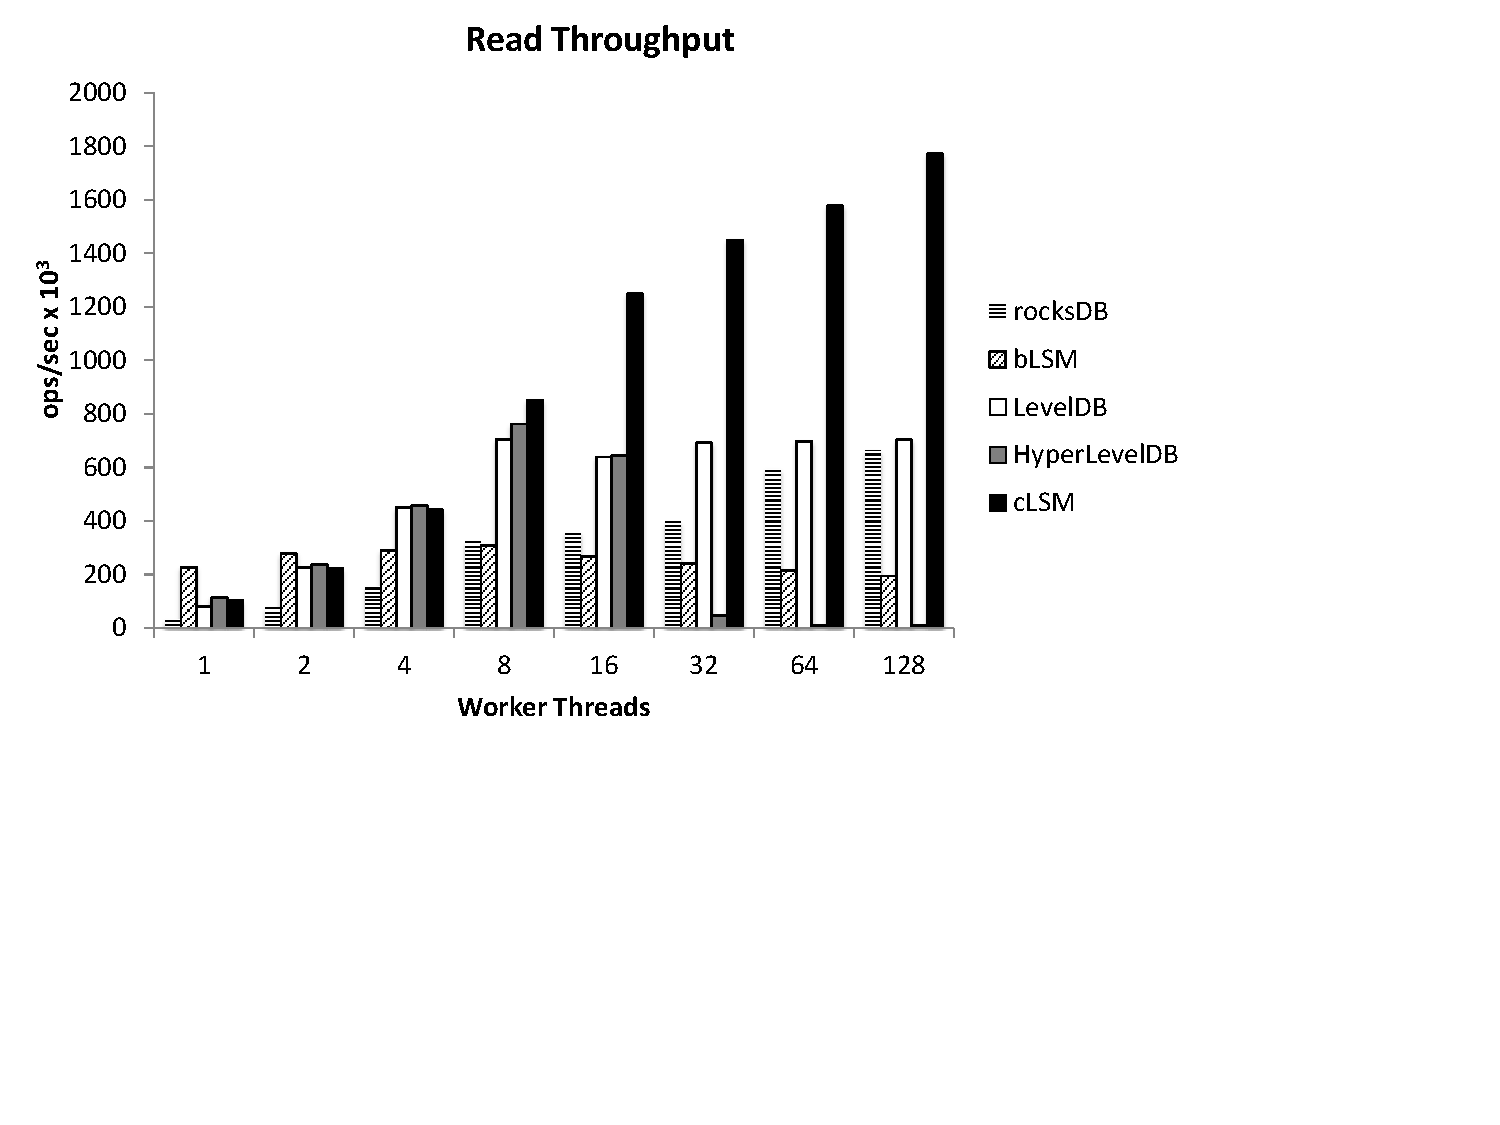
\includegraphics[width=0.9\textwidth,clip, trim =0 180 150 0]{Figures/100_read_throughput.pdf}}
		\caption{Throughput}
               \label{fig:100r_throughput}
  \end{subfigure}%
%\quad
% \hspace{0.2\textwidth}
  \begin{subfigure}[t]{0.49\textwidth}
   \center
        \fbox{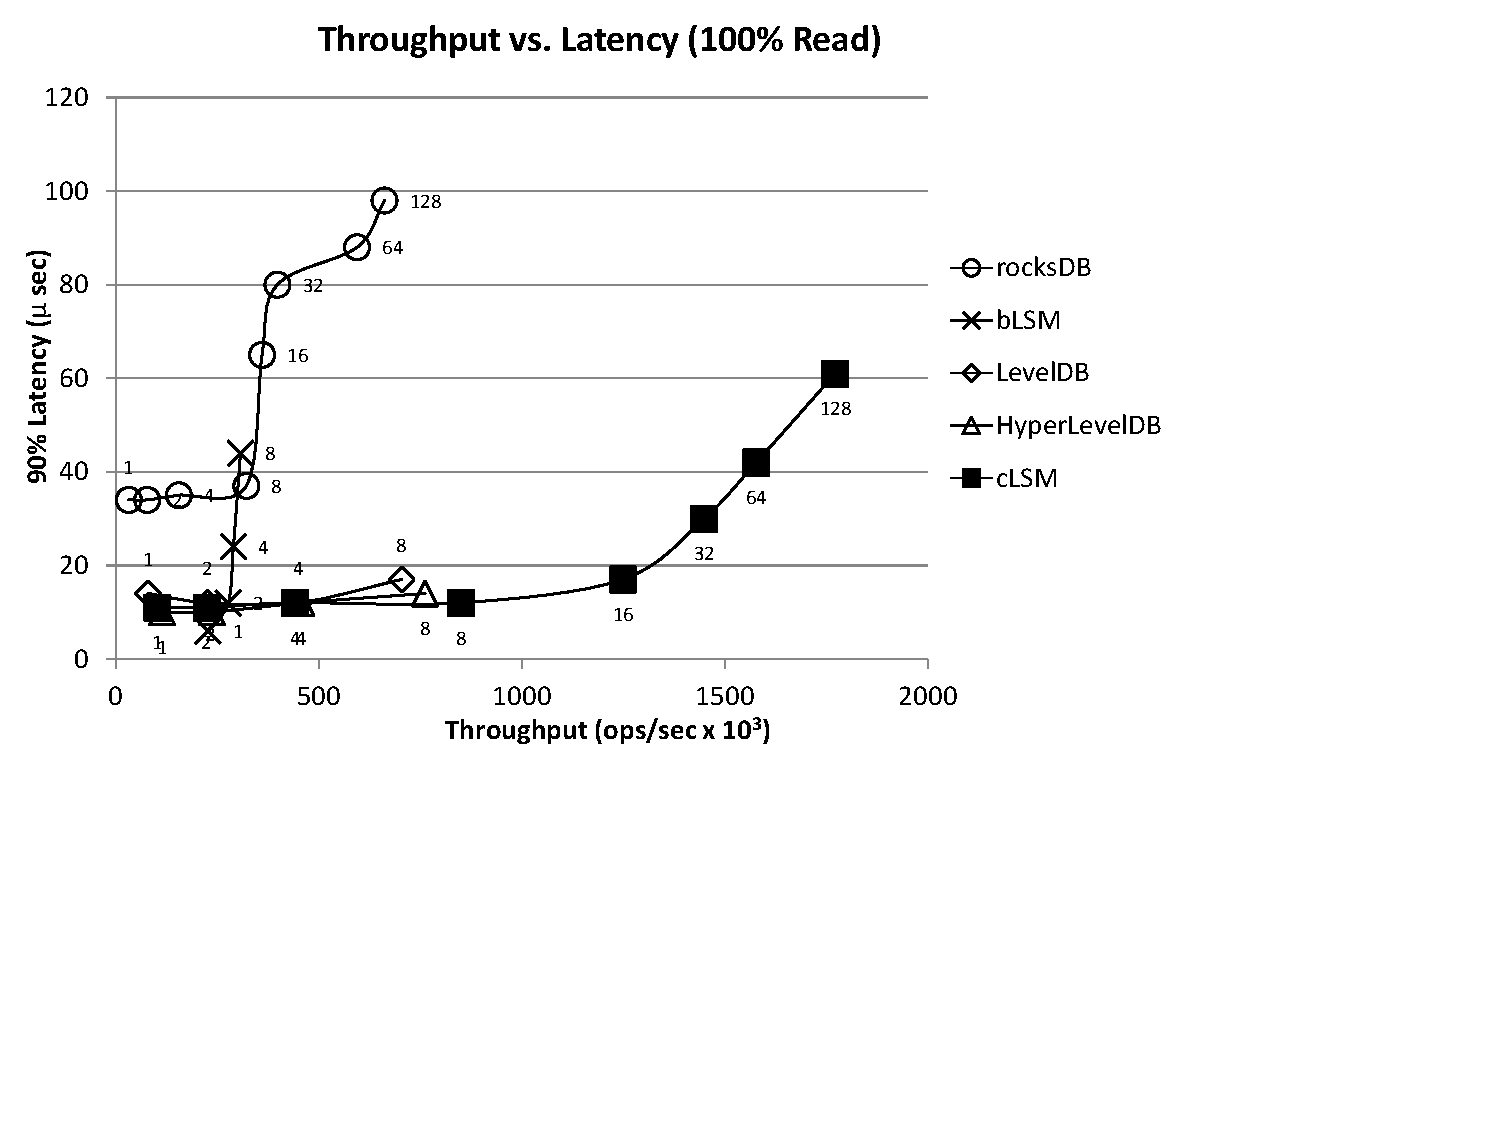
\includegraphics[width=0.9\textwidth,clip, trim =0 180 160 0]{Figures/100_read_latency_vs_throughput.pdf}}
		%{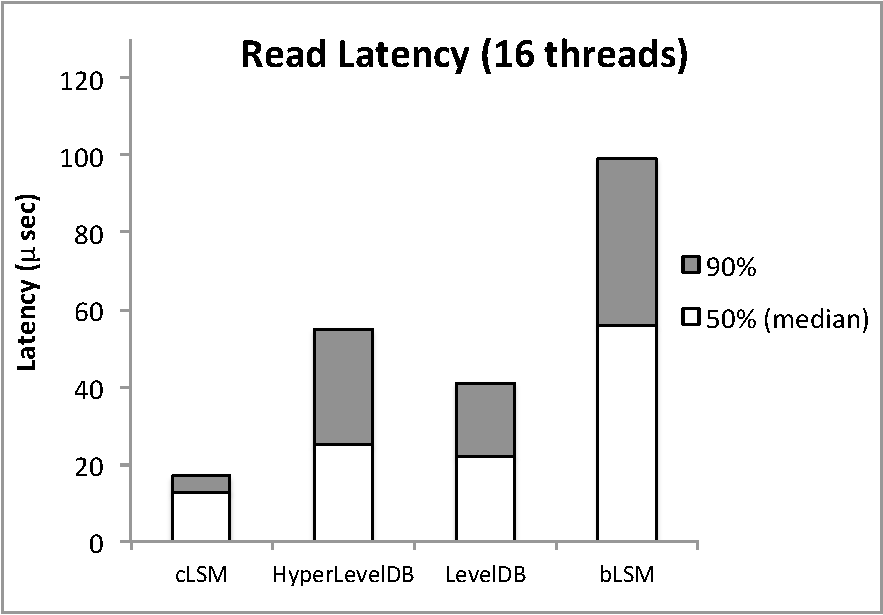
\includegraphics[height=1.8in]{Figures/100_read_16_thread_latency.pdf}}
		\caption{Throughput versus latency; each data point is labeled with the number of threads}
               \label{fig:100r_latencyVSthroughput}
  \end{subfigure}%
\caption{\bf{Read performance -- a 100\% read scenario with locality (90\% of keys picked from 10\% popular blocks).
%{\clsm\/} scales to 128 threads and achieves 130\% throughput advantage over the closest competitor.
}}
\label{fig:100r}
\end{figure*}




{\bf {Mixed workloads.}}
Figure~\ref{fig:50r50w_throughput} depicts the throughput achieved by the different systems
under a 1:1 read-write mix. %The results are consistent with the previous sections.
The original {\leveldb\/} fails to scale, even though the writes are now
only 50\% of the workload.
{\hyperleveldb\/} slightly improves upon that result, whereas {\clsm\/} fully
exploits the software parallelism, scaling beyond 730K operations/sec with 16 workers.

\eurosys{E4}{We note that while under {\clsm\/} and {\hyperleveldb\/} the reads and the writes scale independently (and the throughput numbers are roughly the avarage of the 100\% writes  and 100\% reads scenarios), in  {\leveldb\/} and  {\rocksdb} the writes impede the reads' progress, and therefore the absolute numbers are lower than the average of the 100\% writes  and 100\% reads scenarios.}


Figure~\ref{fig:50scan50w_throughput} repeats the same experiment with reads replaced by range scans.
({\blsm\/} is not part of this evaluation because it does not directly support consistent scans).
The size of each range is picked uniformly between 10 and 20 keys. The number of scan operations is therefore
smaller than the number of writes by an order of magnitude, to maintain the balance between the number
of keys written and scanned. The cumulative throughput is measured as the overall number of accessed keys.
Similarly to the previous cases, the competitors are slower than {\clsm} by more than $60\%$.
\eurosys{E4}{Note that scans are faster than read operations since in each scan operation, the scanned items are located close to the first item, which results in write operations running substantially more than 50\% of the time, and the cross-chip effect causes a small degragation in {\clsm}'s throughput with 16 worker threads.}

\begin{figure*}
  \centering
  \begin{subfigure}[t]{0.49\textwidth}
   \center
        \fbox{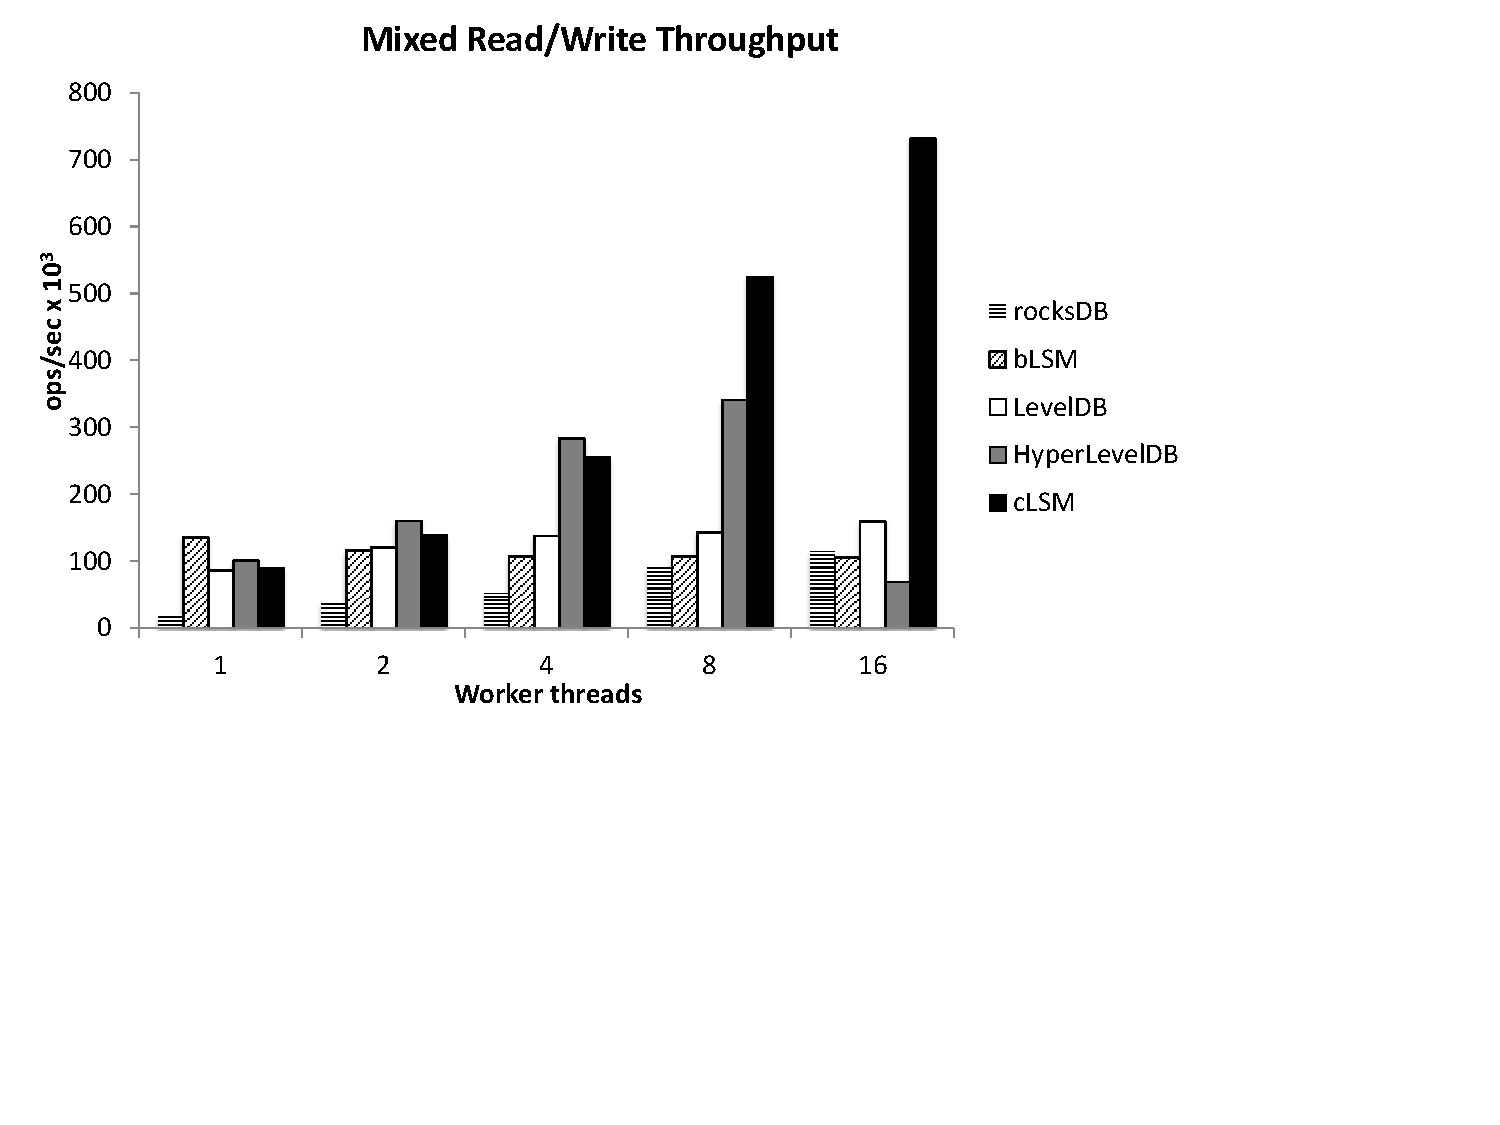
\includegraphics[width=0.9\textwidth,clip, trim =0 180 150 0]{Figures/50r50w_throughput.pdf}}		
		\caption{50\% read, 50\% write}
               \label{fig:50r50w_throughput}
  \end{subfigure}%
%\hspace{0.2\textwidth}
  \begin{subfigure}[t]{0.49\textwidth}
   \center
        \fbox{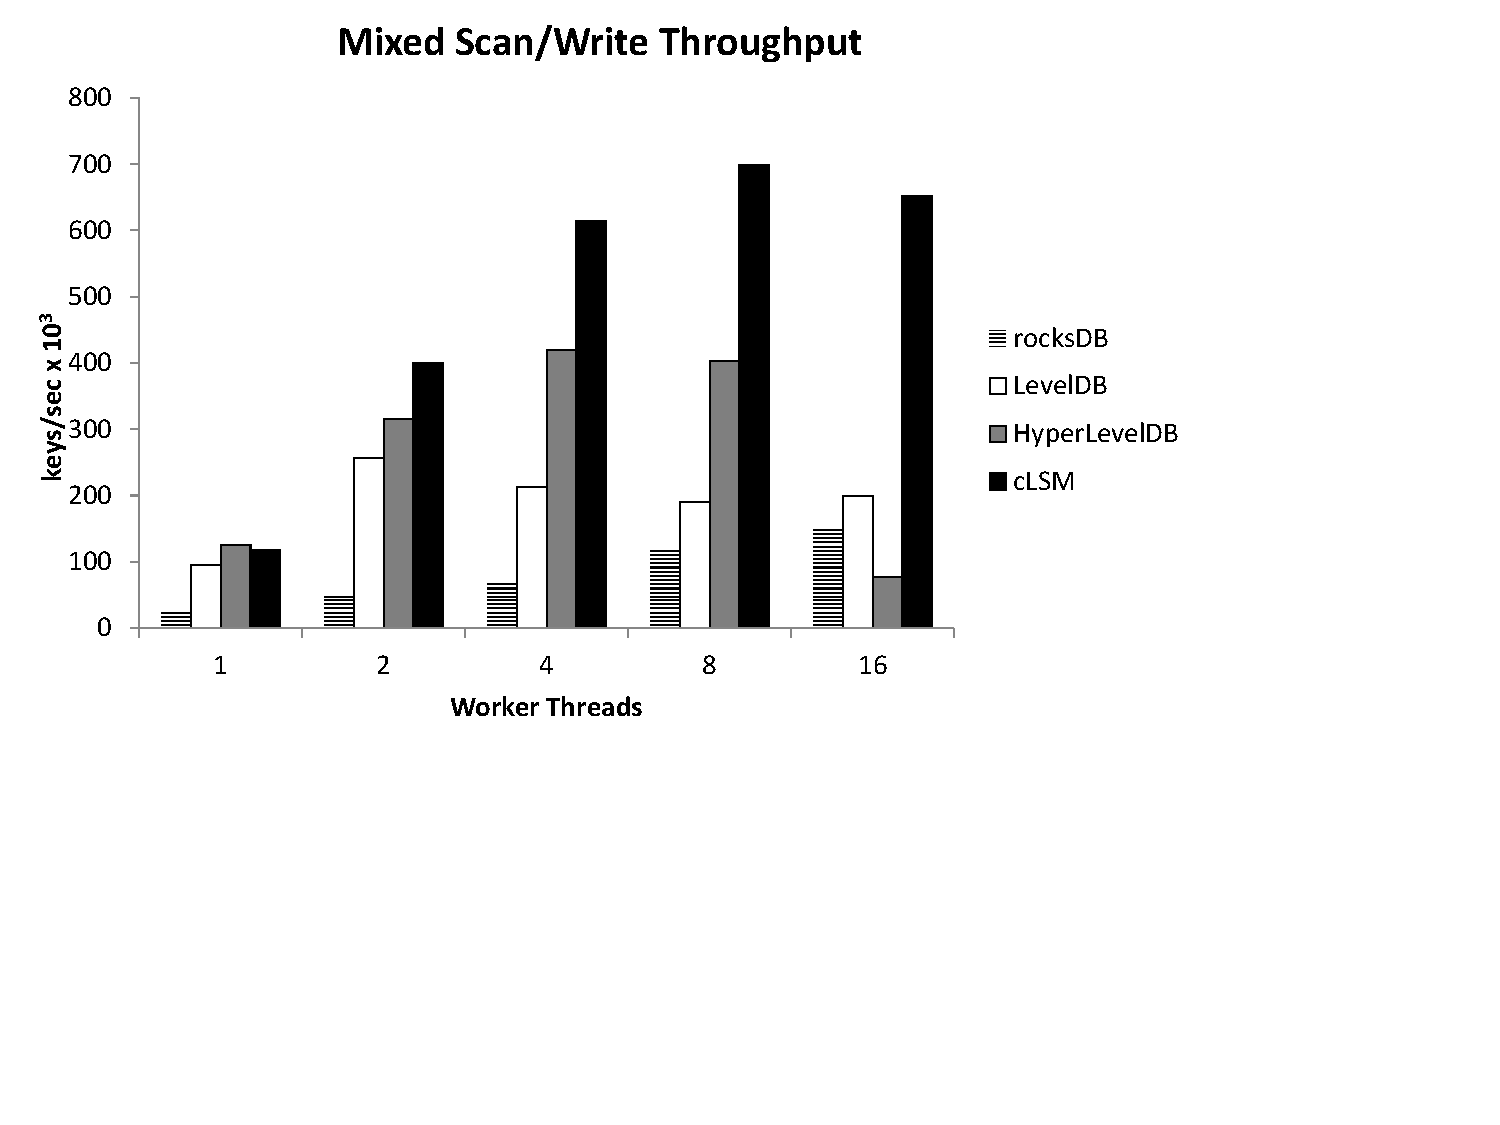
\includegraphics[width=0.9\textwidth,clip, trim =0 180 150 0]{Figures/50scan50w_throughput.pdf}}		
		\caption{50\% scan, 50\% write}
               \label{fig:50scan50w_throughput}
  \end{subfigure}%
\caption{\bf{Throughput in mixed workloads.
%(a) 50\% read/50\% write -- {\clsm}'s peak rate is superior vs the closest competitor by 2.1x. (b) 50\% scan/50\% write --
%{\clsm}'s peak rate (keys per second) is superior by 1.6x.
}}
\label{fig:mixed}
\end{figure*}


We next evaluate how the system may benefit from additional RAM.
%
Figure~\ref{fig:50r50w_buffer} compares {\leveldb}'s and {\clsm}'s benefit from larger memory components,
under the read-write workload, with 8 working threads. {\leveldb\/} performs nearly the same for
all sizes beyond 16MB, whereas {\clsm\/} keeps improving with the memory buffer growing to 512MB.
%This can be explained by the fact that {\clsm} permits several concurrent threads to insert items into the in-memory component,
%whereas in {\leveldb\/} only a single thread may update the in-memory component.
%
%This can be explained as follows.
In general, LSM data stores may gain from increasing the in-memory component
size thanks to better batching of disk accesses~\cite{hbaseRegionArch}. However, this also entails slower in-memory operations. We see that \clsm\ successfully masks this added latency via its high degree of parallelism,
which the less scalable alternatives fail to do.


{\bf {Read-Modify-Write.}}
We now explore the performance of atomic RMW operations (put-if-absent flavor~\cite{shacham2014verifying}).
%None of {\clsm}'s competitors supports the RMW abstraction originally.
To establish a comparison baseline, we augment {\leveldb\/} with a textbook RMW implementation
based on lock striping~\cite{GrayTP1993}. The algorithm  protects each RMW and write
operation with an exclusive granular lock to the accessed key.
The basic read and write implementations remain the same.%, including the concurrency control.

We compare the lock-striped {\leveldb\/} with {\clsm}. The first workload under study is comprised
solely of RMW operations. As shown in Figure~\ref{fig:100rmw_throughput}, {\clsm\/} scales to almost 400K operations/sec -- a $2.5$x
throughput gain compared to the standard implementation.
This volume is almost identical to the peak write load.
%This is explained by  {\clsm}'s high CPU utilization, which allows scaling to 16 threads.
%The median latency with that configuration is 17 {\microsec}, versus {\leveldb}'s 36 {\microsec} (Figure~\ref{fig:100rmw_latency}).


\begin{figure}%[tb]
\centerline{
\fbox{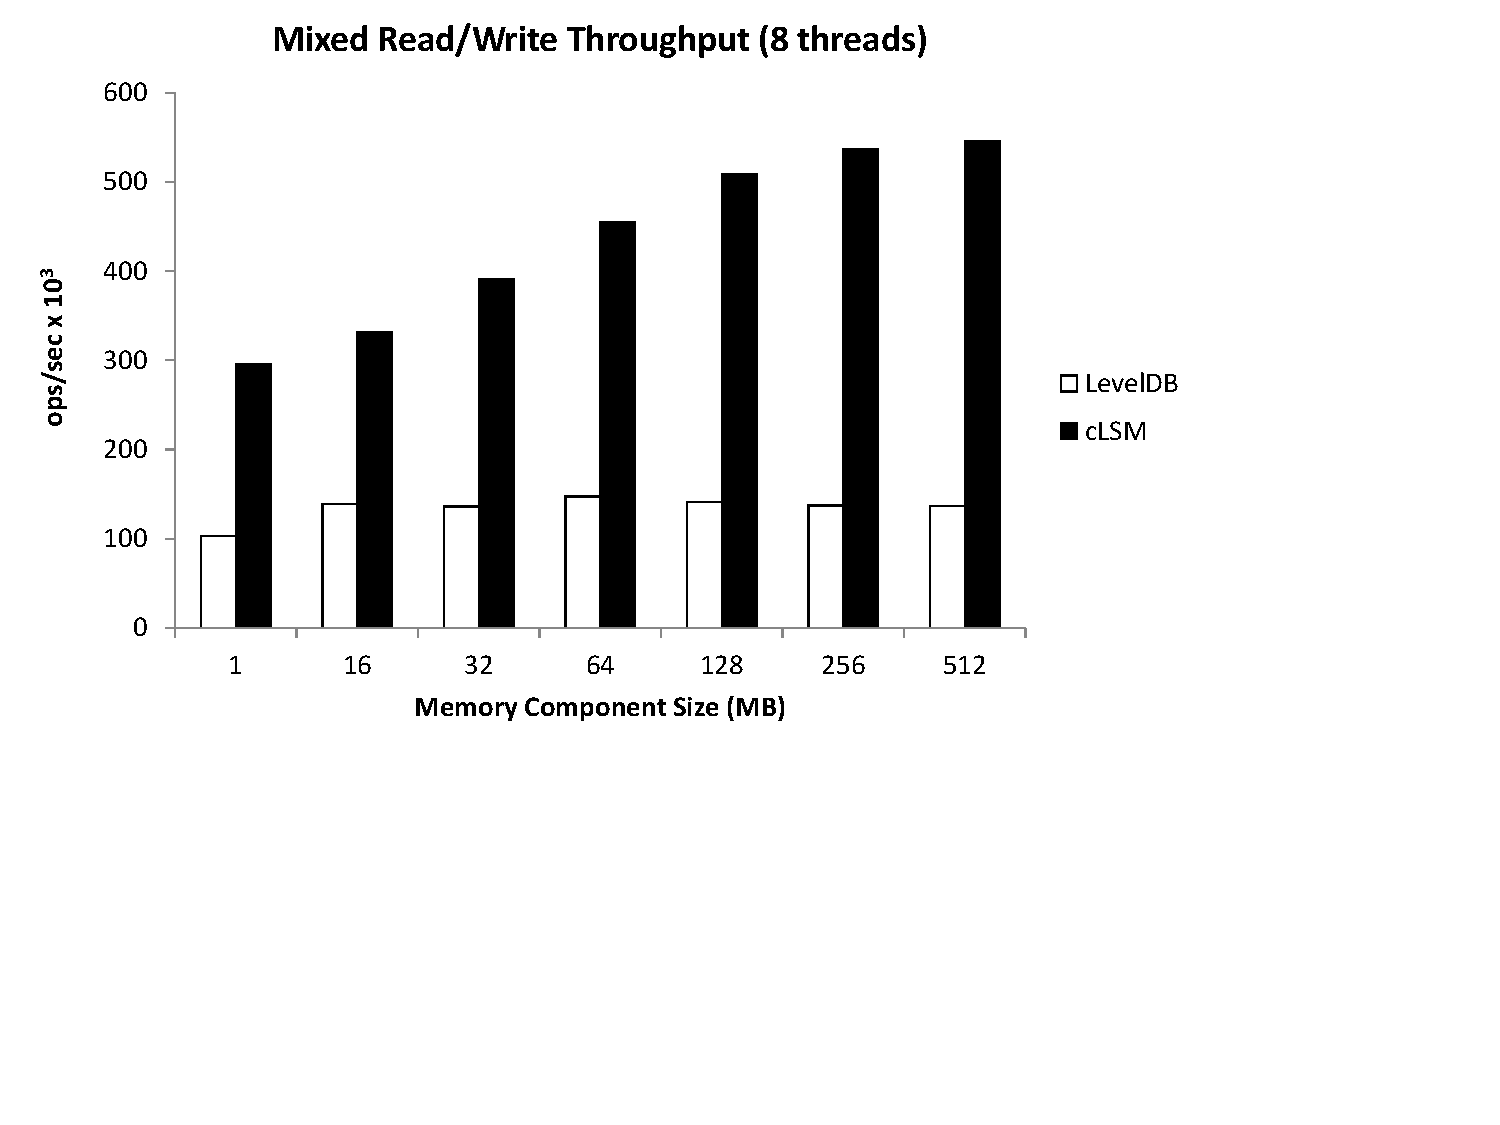
\includegraphics[width=0.45\textwidth,clip, trim =0 180 150 0]{Figures/50r50w_buffer.pdf}}
}
\caption{\bf{Mixed reads and writes benefit from memory component size with 8 threads.
{\clsm\/} successfully exploits RAM buffers of up to 512MB, whereas {\leveldb} can only exploit 16MB. }}
\label{fig:50r50w_buffer}
\end{figure}

\begin{figure}%[tb]
\centerline{
\fbox{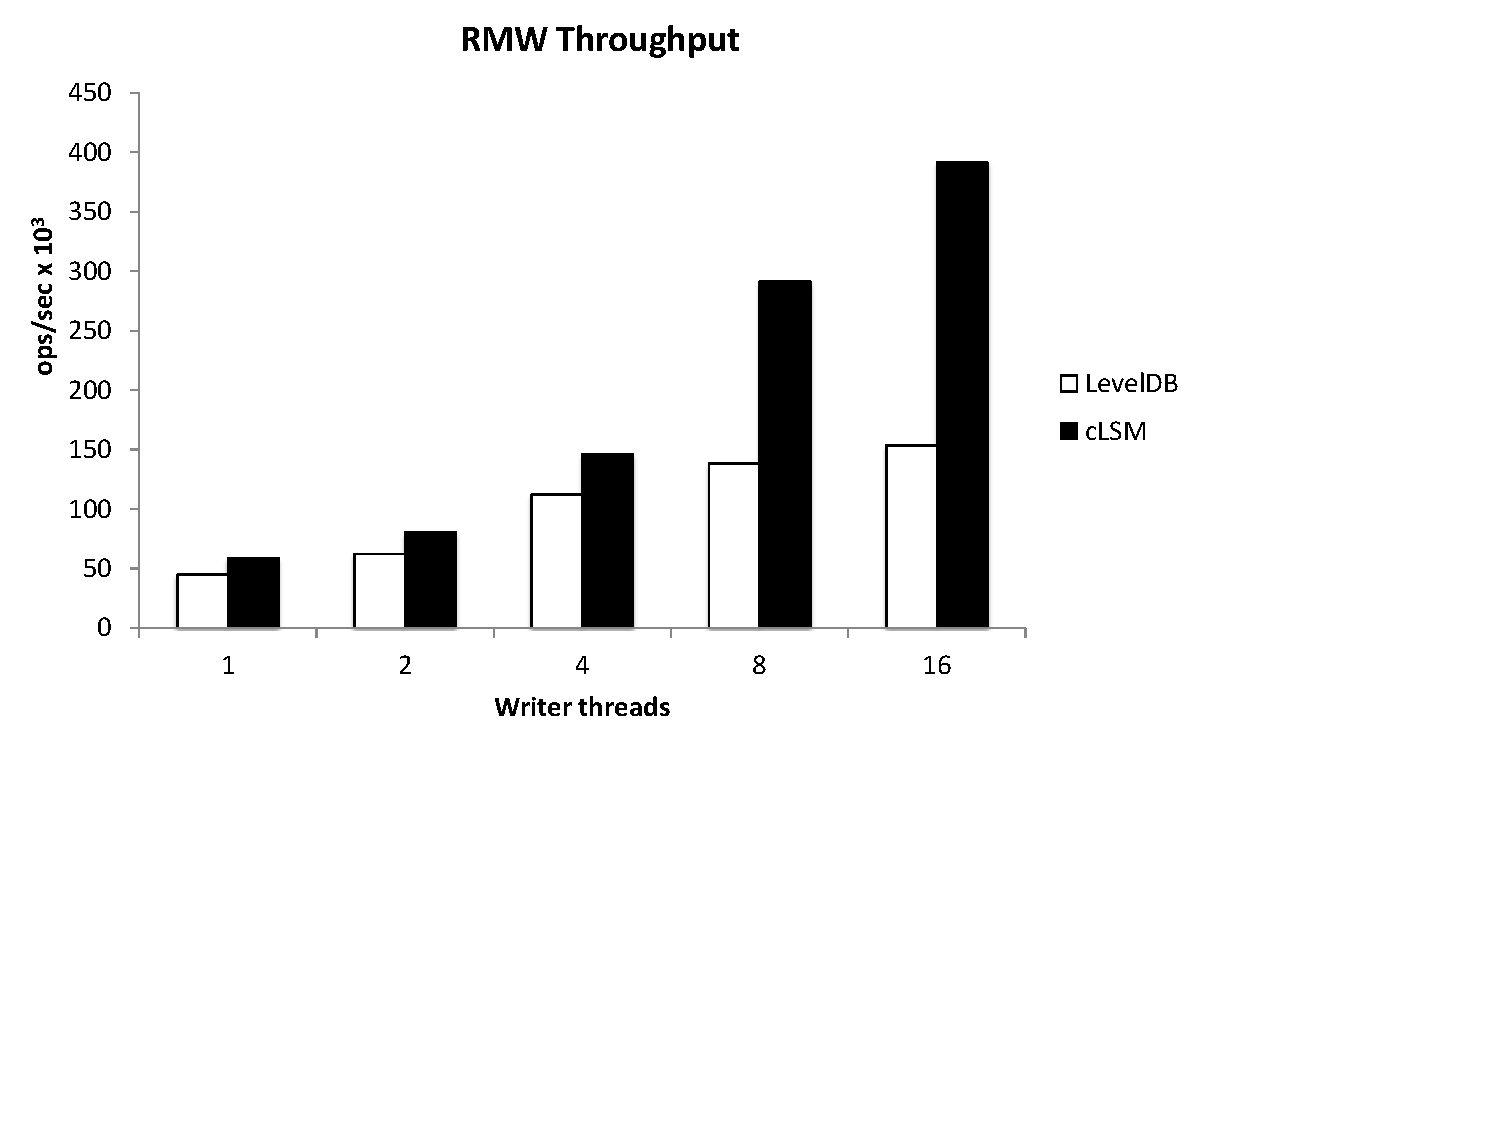
\includegraphics[width=0.45\textwidth,clip, trim =0 180 150 0]{Figures/100_rmw_throughput.pdf}}
}
\caption{\bf{Read-modify-write (RMW) throughput -- a 100\% put-if-absent scenario with locality.
{\clsm\/} improves upon lock-striping by 150\%.}}
\label{fig:100rmw_throughput}
\end{figure}

%\begin{figure*}[tb]
%  \centering
%  \begin{subfigure}[t]{0.49\textwidth}
%   \center
%        \fbox{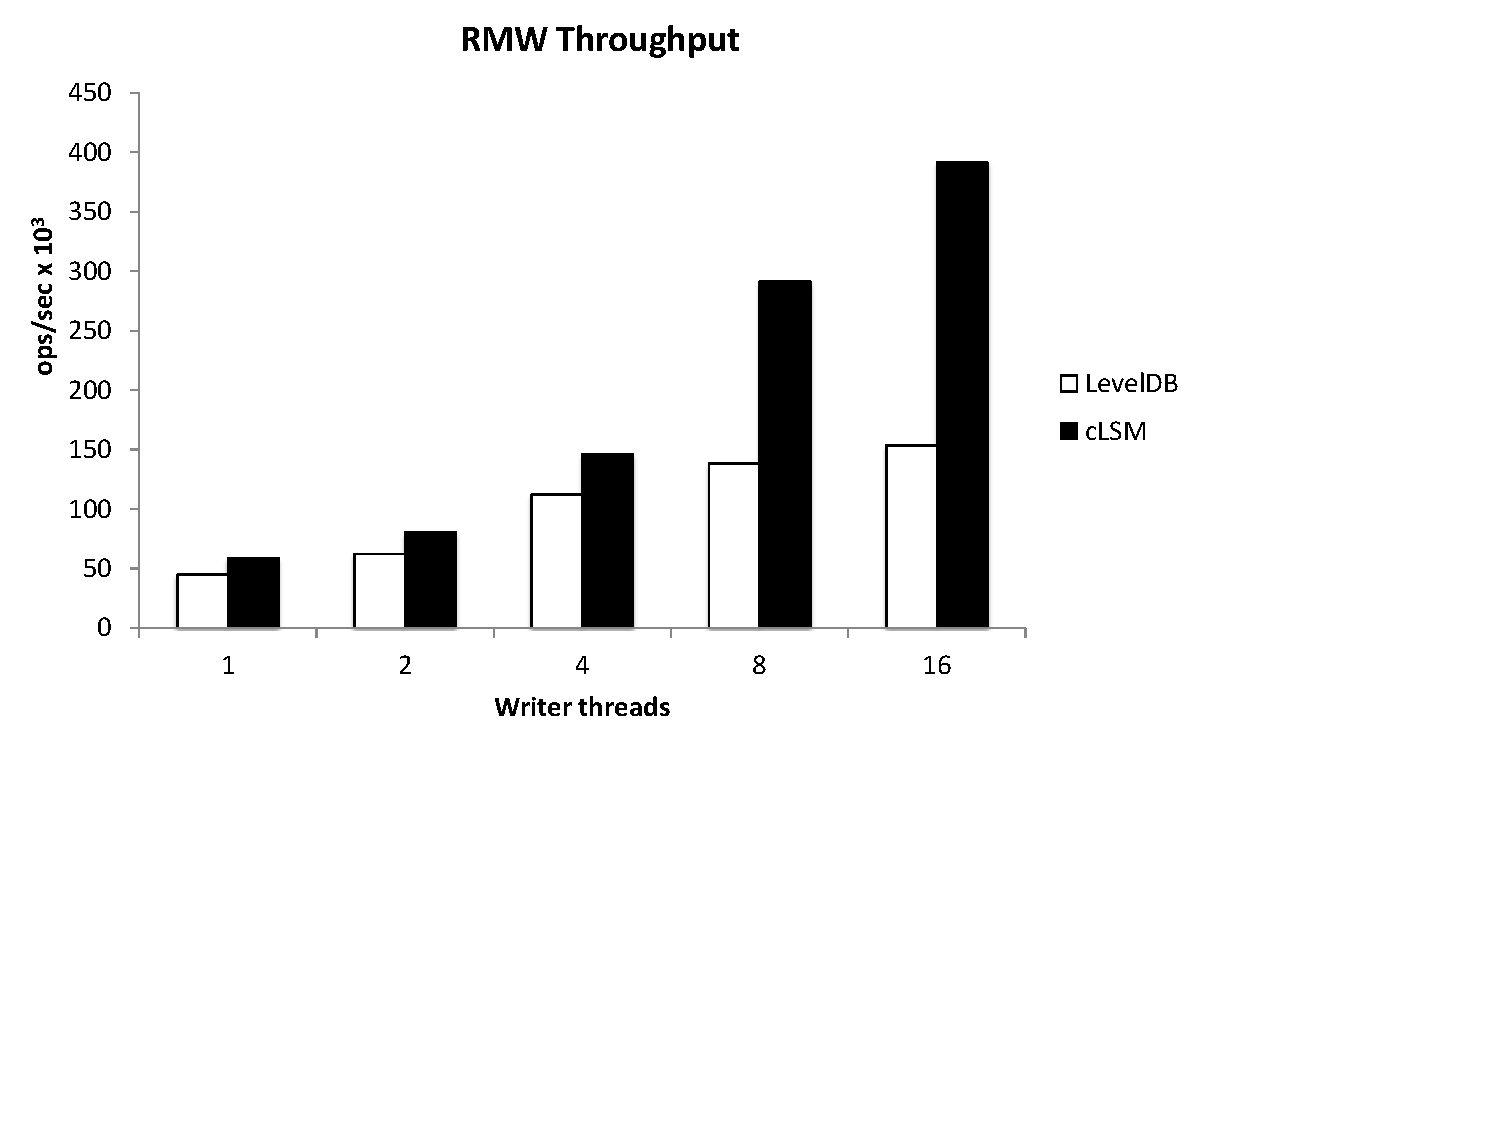
\includegraphics[width=0.9\textwidth,clip, trim =0 180 165 0]{Figures/100_rmw_throughput.pdf}}
%		\caption{Throughput}
%               \label{fig:100rmw_throughput}
%  \end{subfigure}%
%%\quad
% %\hspace{0.2\textwidth}
%  \begin{subfigure}[t]{0.49\textwidth}
%   \center
%		\fbox{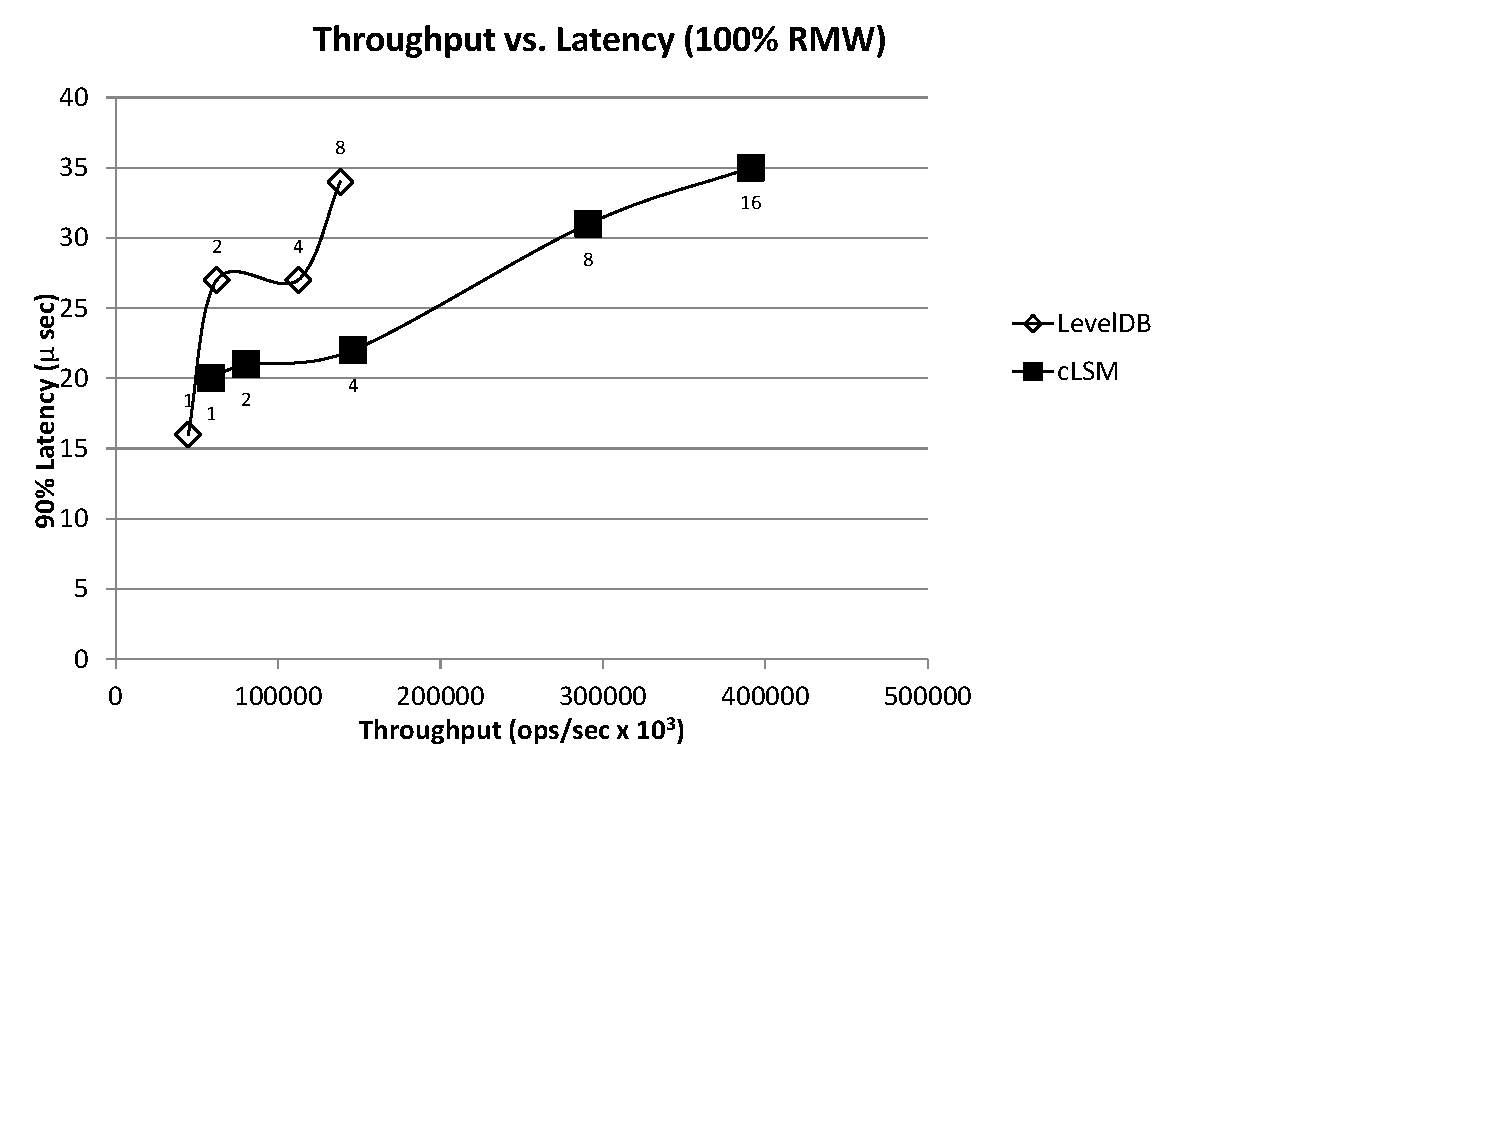
\includegraphics[width=0.9\textwidth,clip, trim =0 180 165 0]{Figures/100_rmw_latency_vs_throughput.pdf}}
%		\caption{Throughput versus Latency}
%               \label{fig:100rmw_latency}
%  \end{subfigure}%
%\caption{\bf{Read-modify-write (RMW) performance -- a 100\% put-if-absent scenario with locality.
%{\clsm\/} exceeds the na\"{\i}ve lock-striping throughput by 150\%, and
%has superior median and 90\% latencies.}}
%\label{fig:100rmw}
%\end{figure*}

%{\bf {Disk Activity.}}
%In the above experiments, the {\clsm} performance can be explained by its effective in-memory synchronization.
%In order to understand the behaviour of the {\clsm}'s disk-component, we measure the amount of time the \emph{compaction procedures} are running
%(as described in Section~\ref{ssec:lsm}, compactions are used to rearrange the internal components of the disk-component).
%Figure~\ref{fig:CompactionsExecution} shows the percentage of execution time in which compactions are running in our experiments.
%The results indicate that, in most cases, compactions are running for at least $50\%$ of the execution time.
%Note that, {\clsm}'s compactions are executed by a single background thread (the implementation of the disk compactions has been taken from {\leveldb}).
%
%\begin{figure}
%\footnotesize
%\begin{tabular}{ c | c }
%%  Workload & Average $\%$ time compaction is running   \\
%  Workload & Average $\%$ time    \\
%           & compactions are running in the background  \\
%  \hline
%  100\% write & 65\%   \\
%  100\% read & 49\%   \\
%  50\% write, 50\% read & 75\%   \\
%\end{tabular}
%\caption{\bf{Execution time of compactions in {\clsm}.}}
%\label{fig:CompactionsExecution}
%\end{figure}



\subsection{Production Workloads}
\label{sec:realworkloads}

\begin{figure*}[tb]
  \centering
  \begin{subfigure}[t]{0.4\textwidth}
   \center
        \fbox{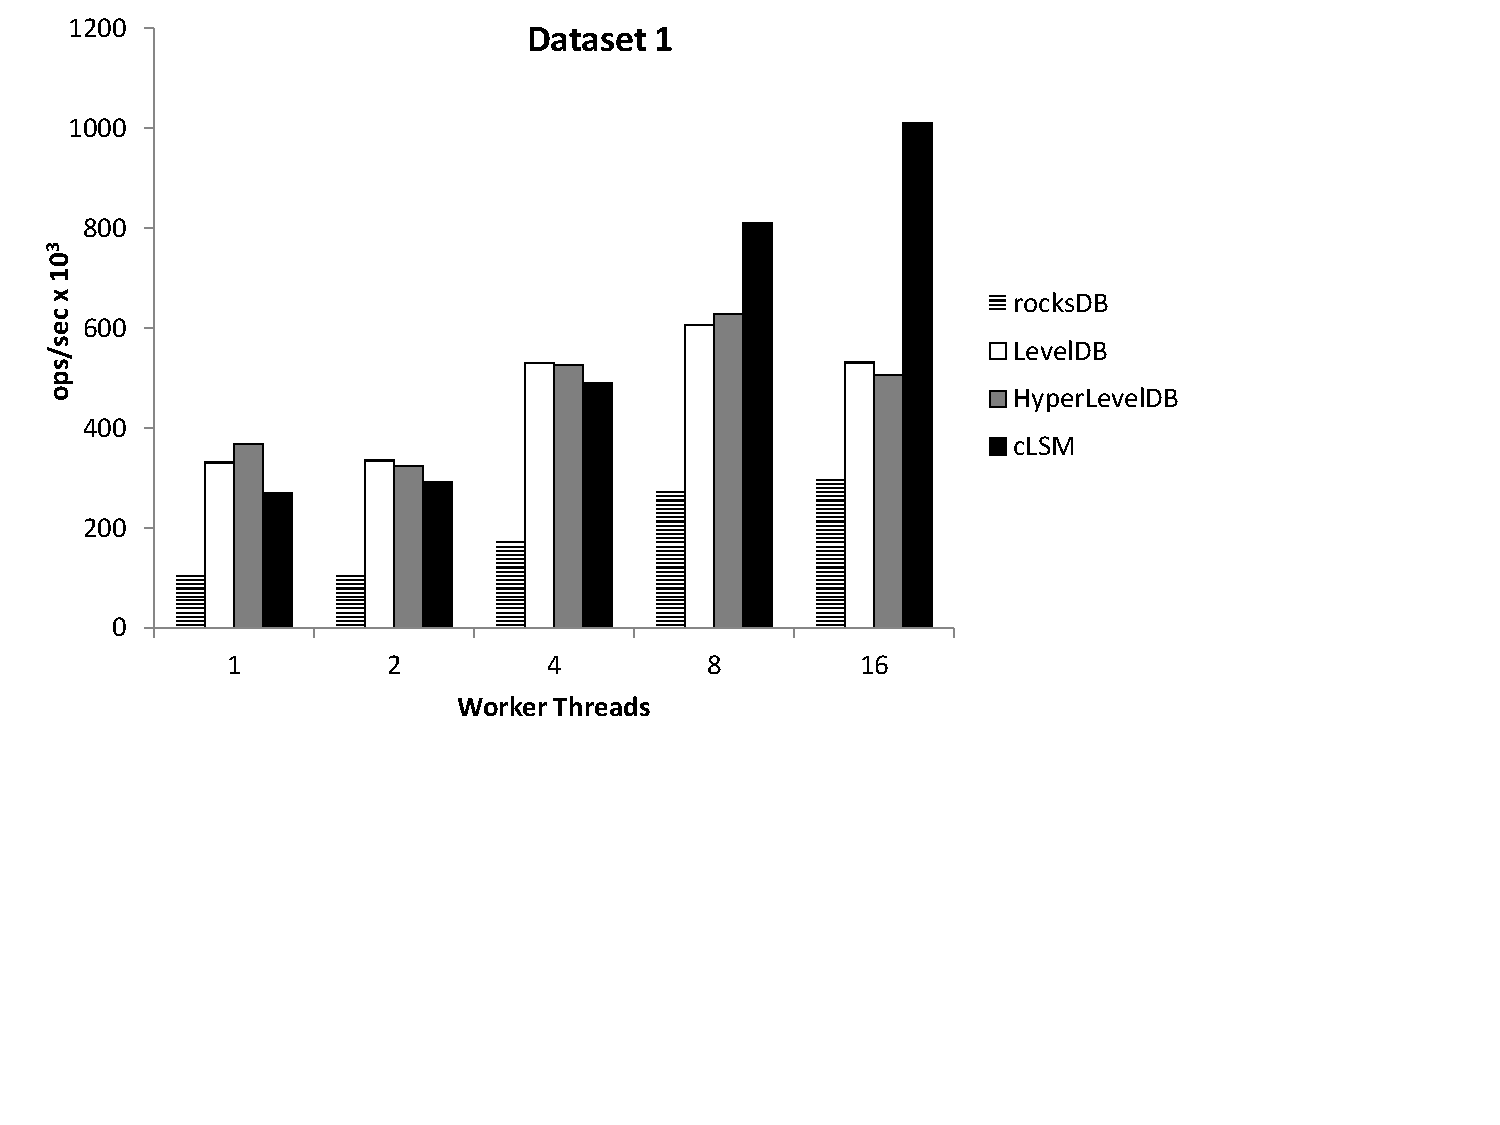
\includegraphics[width=0.9\textwidth,clip, trim =0 180 155 0]{Figures/prodA.pdf}}	
		\caption{93\% reads}
               \label{fig:prodA}
  \end{subfigure}%
%\quad
 %\hspace{0.05\textwidth}
  \begin{subfigure}[t]{0.4\textwidth}
   \center
        \fbox{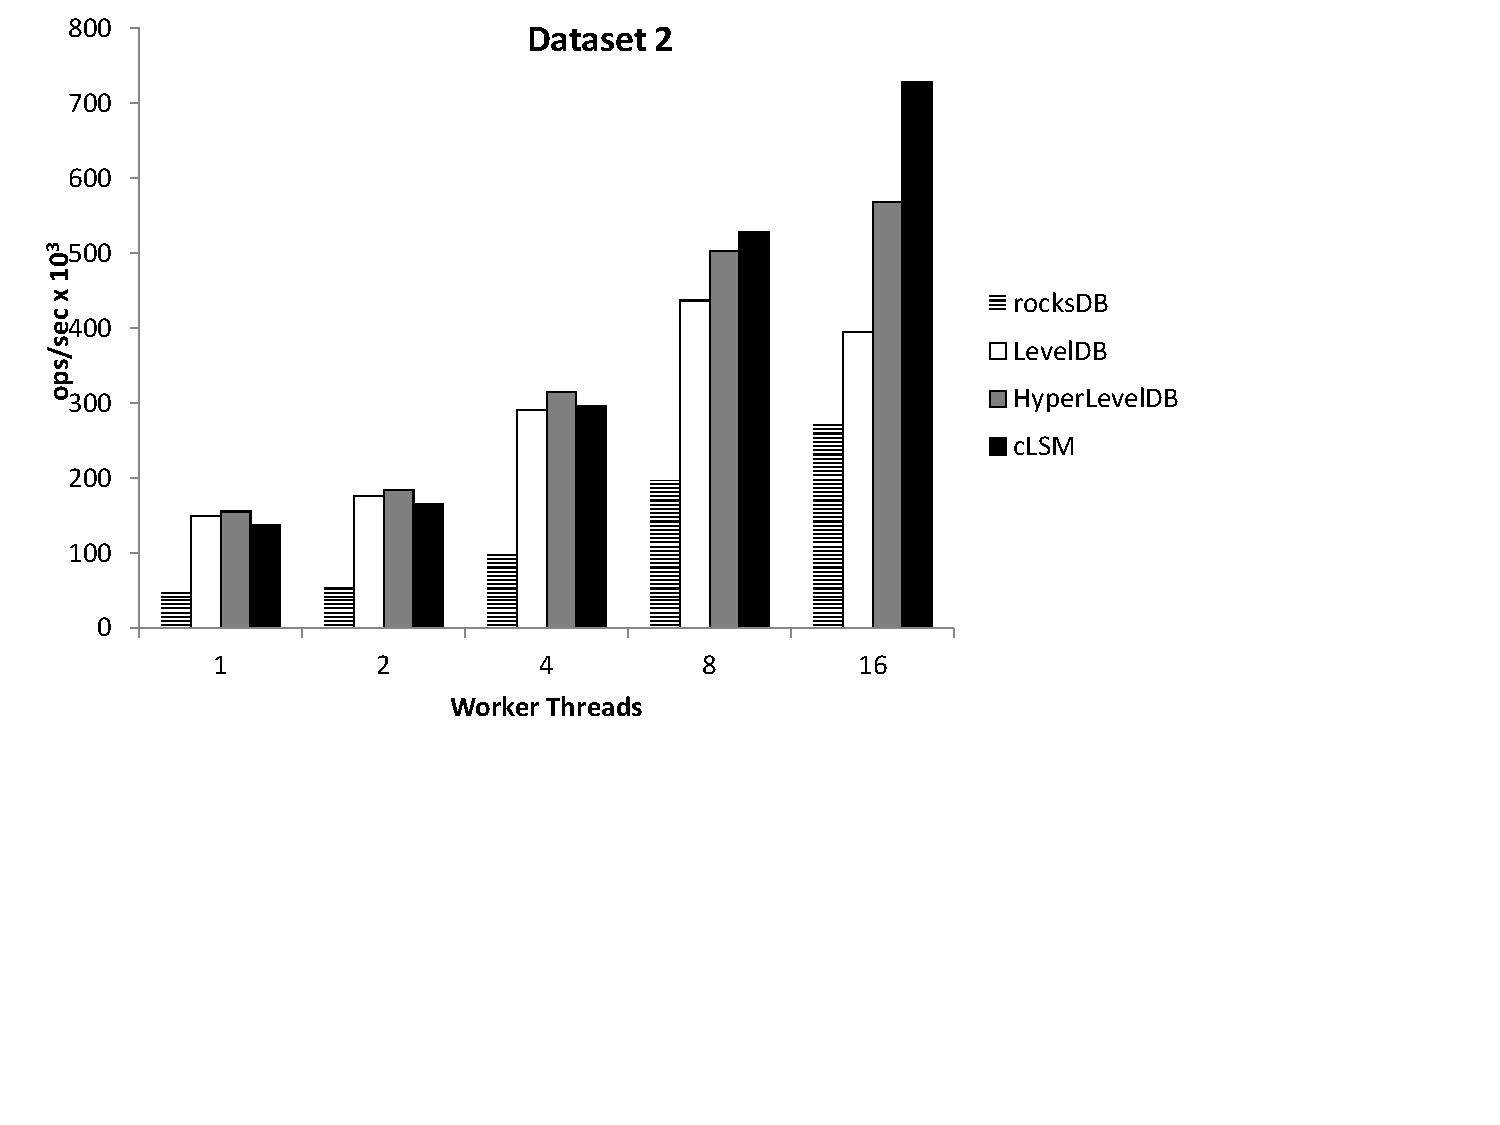
\includegraphics[width=0.9\textwidth,clip, trim =0 180 155 0]{Figures/prodB.pdf}}
		\caption{85\% reads}
               \label{fig:prodB}
  \end{subfigure}%
\hfill
  \centering
  \begin{subfigure}[b]{0.4\textwidth}
   \center
        \fbox{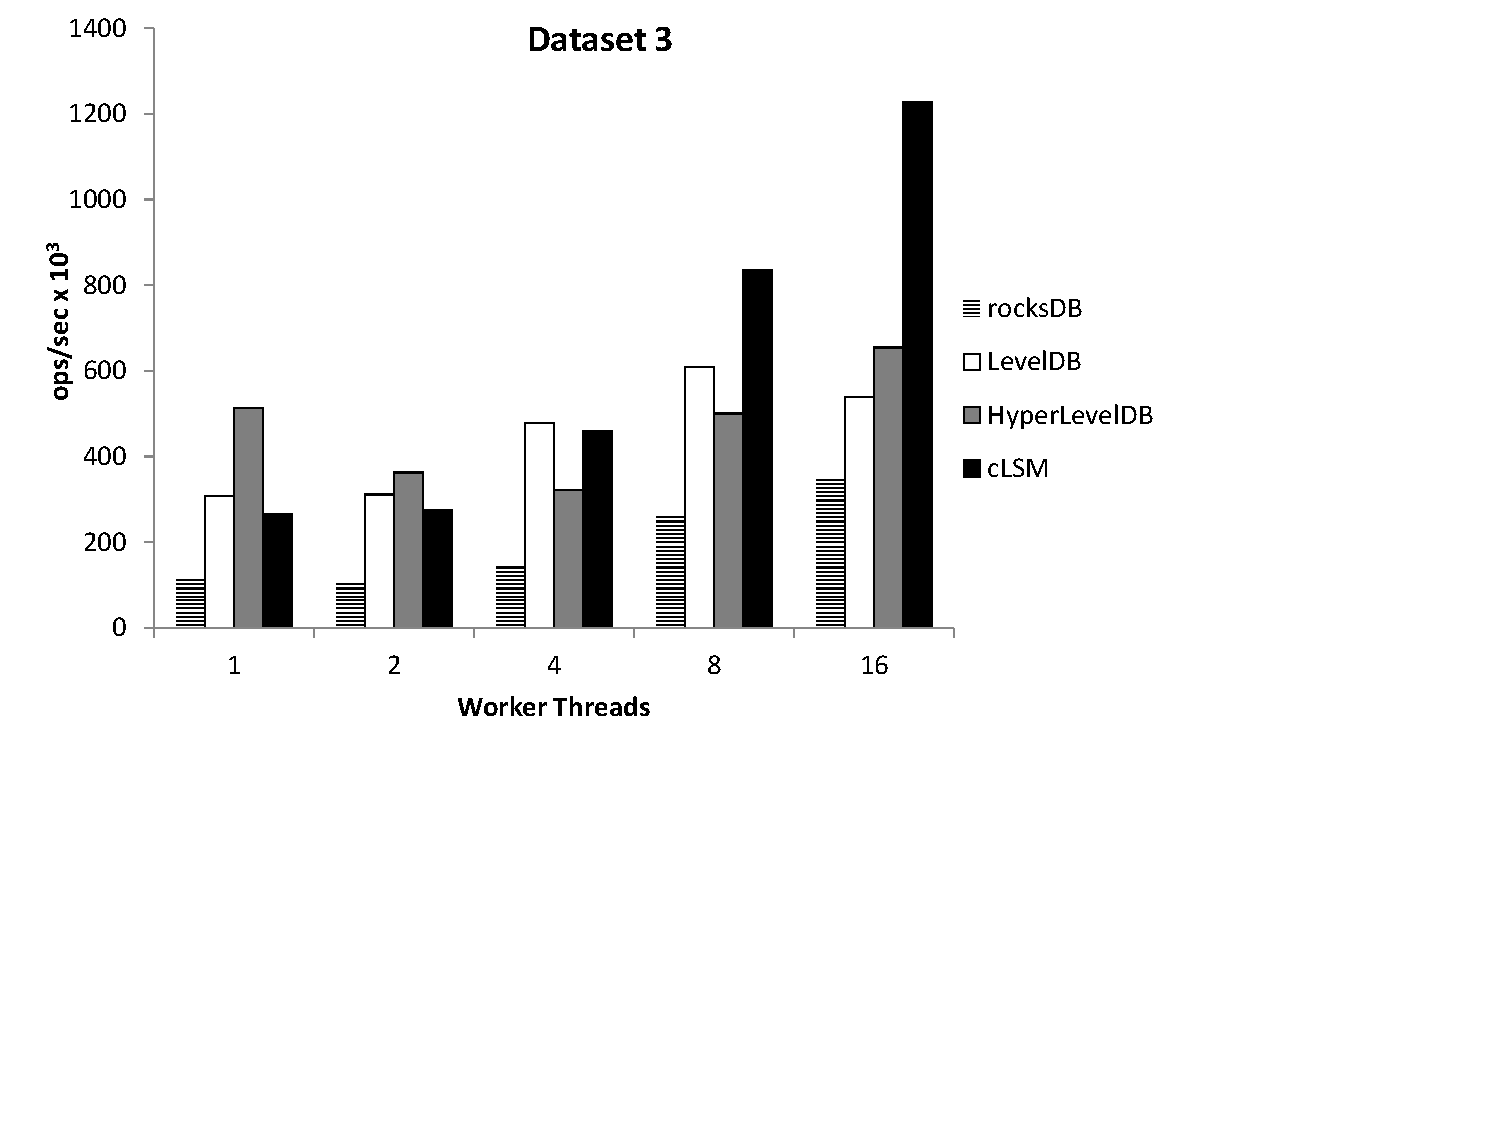
\includegraphics[width=0.9\textwidth,clip, trim =0 180 155 0]{Figures/prodD.pdf}}
		\caption{96\% reads}
               \label{fig:prodD}
  \end{subfigure}%
%\quad
 %\hspace{0.05\textwidth}
  \begin{subfigure}[b]{0.4\textwidth}
   \center
        \fbox{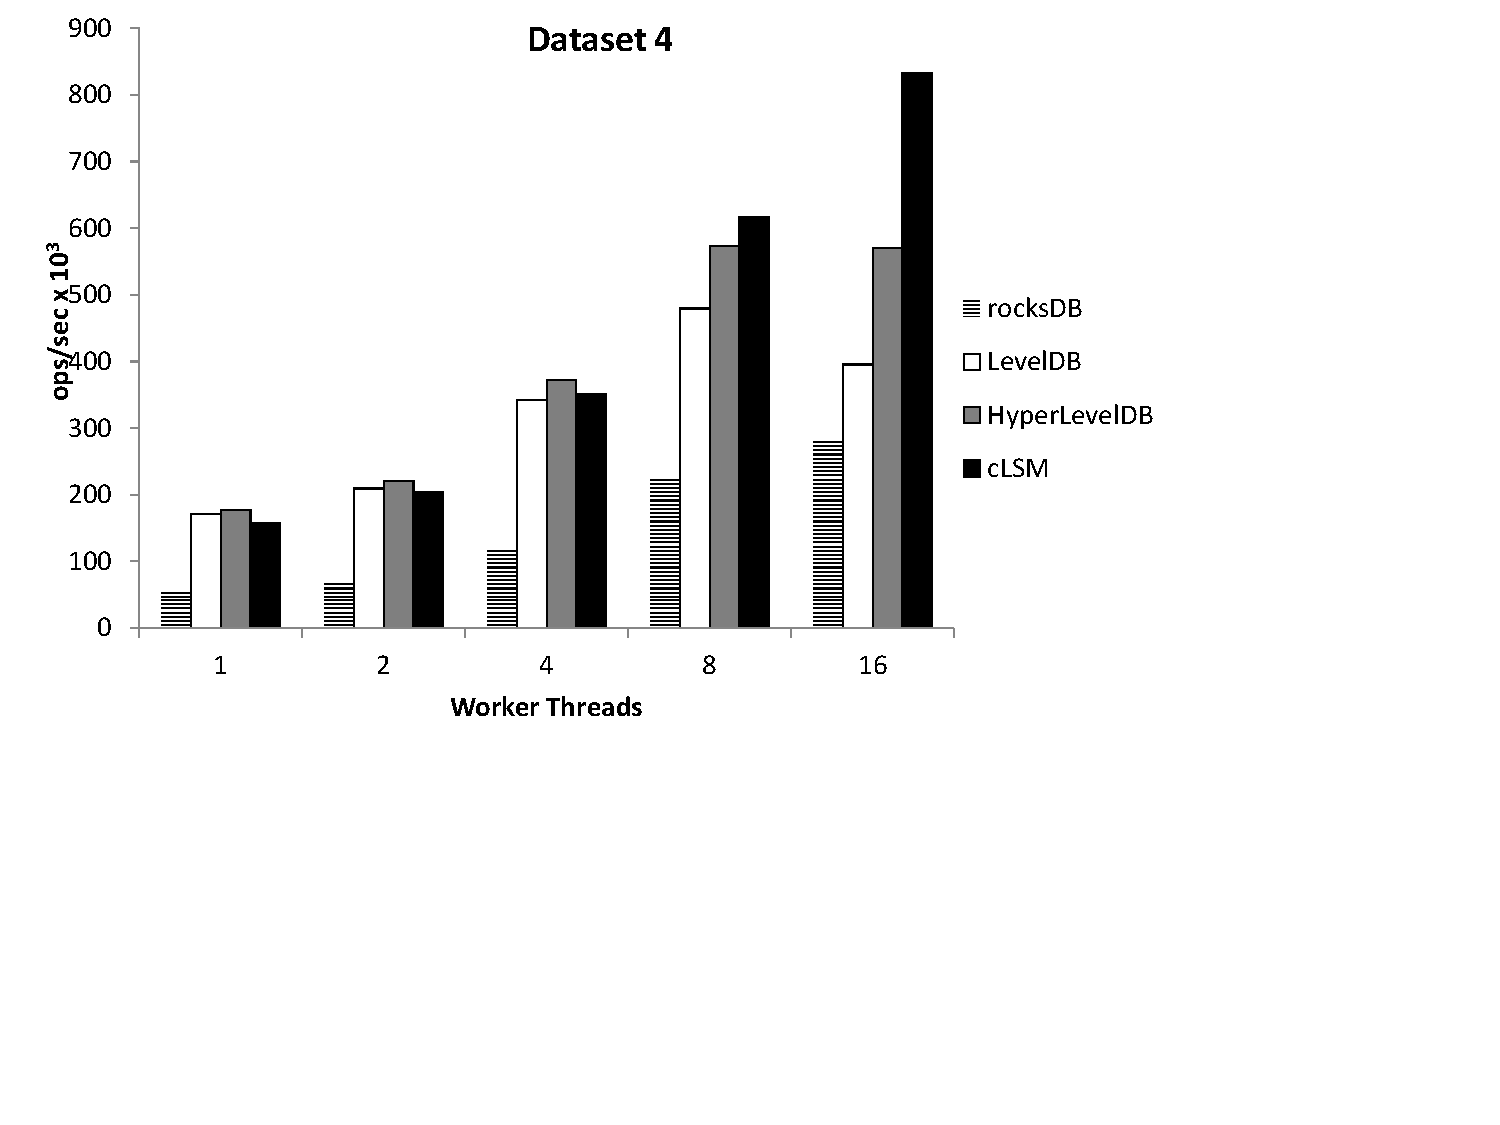
\includegraphics[width=0.9\textwidth,clip, trim =0 180 155 0]{Figures/prodE.pdf}}
		\caption{86\% reads}
               \label{fig:prodE}
  \end{subfigure}%
\caption{\bf{
Throughput in workloads collected from a production web-scale system.
}}
\label{fig:production}
\end{figure*}

We study a set of $20$ workloads logged in a production key-value store that
serves some of the major personalized content and advertising systems on the web. Each log captures the
history of operations applied to an individual partition server. The average
log consists of approximately 5 million operations.
\eurosys{E1}{Operations have variable key and value sizes, averaging $40$-bytes per key, and 1KB
values.} The captured workloads are read-dominated (85\% to 95\% reads).  The key distributions are heavy-tail,
all with similar locality properties. In most settings, 10\% of the keys stand for more than 75\% of the requests,
while the 1-2\% most popular keys account for more than 50\%. Approximately 10\% of the keys are only
encountered once.


Figure~\ref{fig:production} depicts the evaluation results for 4 representative workloads.
Although {\clsm} is slower than the alternatives with a small number of
threads, its scalability is much better.
These results are similar to the results shown in~\ref{fig:50r50w_throughput}.
\eurosys{E1}{However, our advantage over
the competitors is reduced, because, with larger keys and values, the
synchronization overhead is less pronounced.}




\remove{
We also use the logs to conduct an  experiment that compares two approaches to vertical scalability.
We evaluate {\clsm\/} with one big partition versus {\leveldb\/} and {\hyperleveldb\/} with four small partitions.
%Recall that, in many cases, the former setting is more efficient from the I/O perspective~\cite{hbaseRegionArch}.
In this experiment, each small partition
is based on a distinct log, and the big partition is a union thereof.  Each of the small partitions is served
by a dedicated $1/4$ of the thread pool (resource separation), whereas the big partition is served by all
worker threads (resource sharing).
Figure~\ref{fig:production_partitions} depicts the comparison.
We see that {\clsm\/}'s improved concurrency control scales better than partitioning, achieving a peak throughput of above 1 million operations/sec -- approximately 25\% above the competition.
%
This suggests that vertical scalability can sometimes go further than increased horizontal scaling.


\begin{figure}[tbh]
\centerline{
{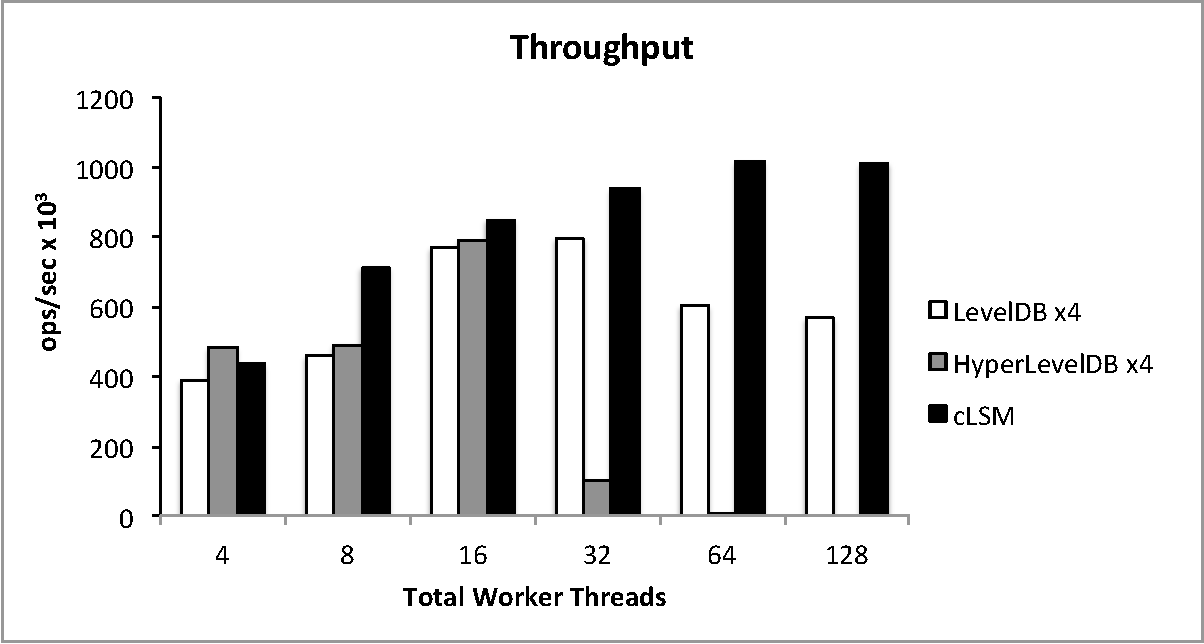
\includegraphics[width=\columnwidth]{Figures/prod4Partitions.pdf}}
}
\caption{\bf{Production workload -- comparing two approaches to vertical scalability.
The resource-isolated configuration exercises {\leveldb\/} and {\hyperleveldb\/} with
4 separate partitions, whereas the resource-shared configuration evaluates {\clsm\/} with
one big partition.
%{\clsm} scales 25\% beyond the competition.
}}
\label{fig:production_partitions}
\end{figure}
}


\subsection{Workloads with Heavy Disk-Compaction}
\label{sec:heavyCompaction}

The above experiments demonstrate situations in which the in-memory access is the main performance bottleneck.
Recently, the {\rocksdb} project has shown that in some scenarios, the main  performance bottleneck is  disk-compaction~\cite{RocksDBBenchmarks}.
%
In these scenarios, a huge number of items is inserted (at once) into the LSM store, leading to many heavy disk-compactions.
As a result of the high disk activity, the  $C_{m}$ component frequently becomes full before the $C_{m}'$ component has been merged into the disk.
This causes client operations to wait until the merge process completes.

We use a benchmark from~\cite{RocksDBBenchmarks} to demonstrate this situation.
In this benchmark, the initial database is created by sequentially inserting 1 billion items.
During the benchmark, 1 billion update operations are invoked by the worker threads.
\eurosys{E3}{As in~\cite{RocksDBBenchmarks}, each key is of size $10$
bytes; however, each value is of size $400$ bytes (instead of $800$)} to ensure that our $720$GB disk is sufficient.


We compare {\clsm} with {\rocksdb} \eurosys{E3}{following the configuration
in~\cite{RocksDBBenchmarks}.
% For {\rocksdb}, we use the configuration in~\cite{RocksDBBenchmarks}.
{\rocksdb} is configured to use multi-threaded compactions so that multiple
threads can simultaneously compact non-overlapping key
ranges in multiple levels.
%For {\clsm}, we adopt part of the {\rocksdb} configuration:
%
%although {\clsm} and {\rocksdb} have different configurable parameters,
%some of these parameters appear in both configurations;
For each parameter that appears both in {\clsm} and {\rocksdb}, we configure the
systems to use the same values.
Specifically, these parameters are: size of
in-memory component ($128$MB), total number of levels ($6$ levels), target file size at level-1 ($64$MB),
and number of bytes in a block ($64$KB).
}

Figure~\ref{fig:HeavyCompactions} depicts the results of this benchmark.
The results show that both {\clsm} and  {\rocksdb}  scale all the way to $16$ worker threads (despite the fact that disk-compaction is running most of the time).
At $16$ threads, {\clsm} becomes equivalent to {\rocksdb}.
Notice that {\rocksdb} uses an optimized compaction algorithm  that utilizes several background threads,
whereas {\clsm} uses a simpler compaction algorithm executed by a single background thread.
It should be noted that {\rocksdb}'s compaction optimizations are orthogonal to our improved parallelism among worker threads.

%\remove{
%eshcar - moved to related.tex for placment
\begin{figure}[t]
\centerline{
\fbox{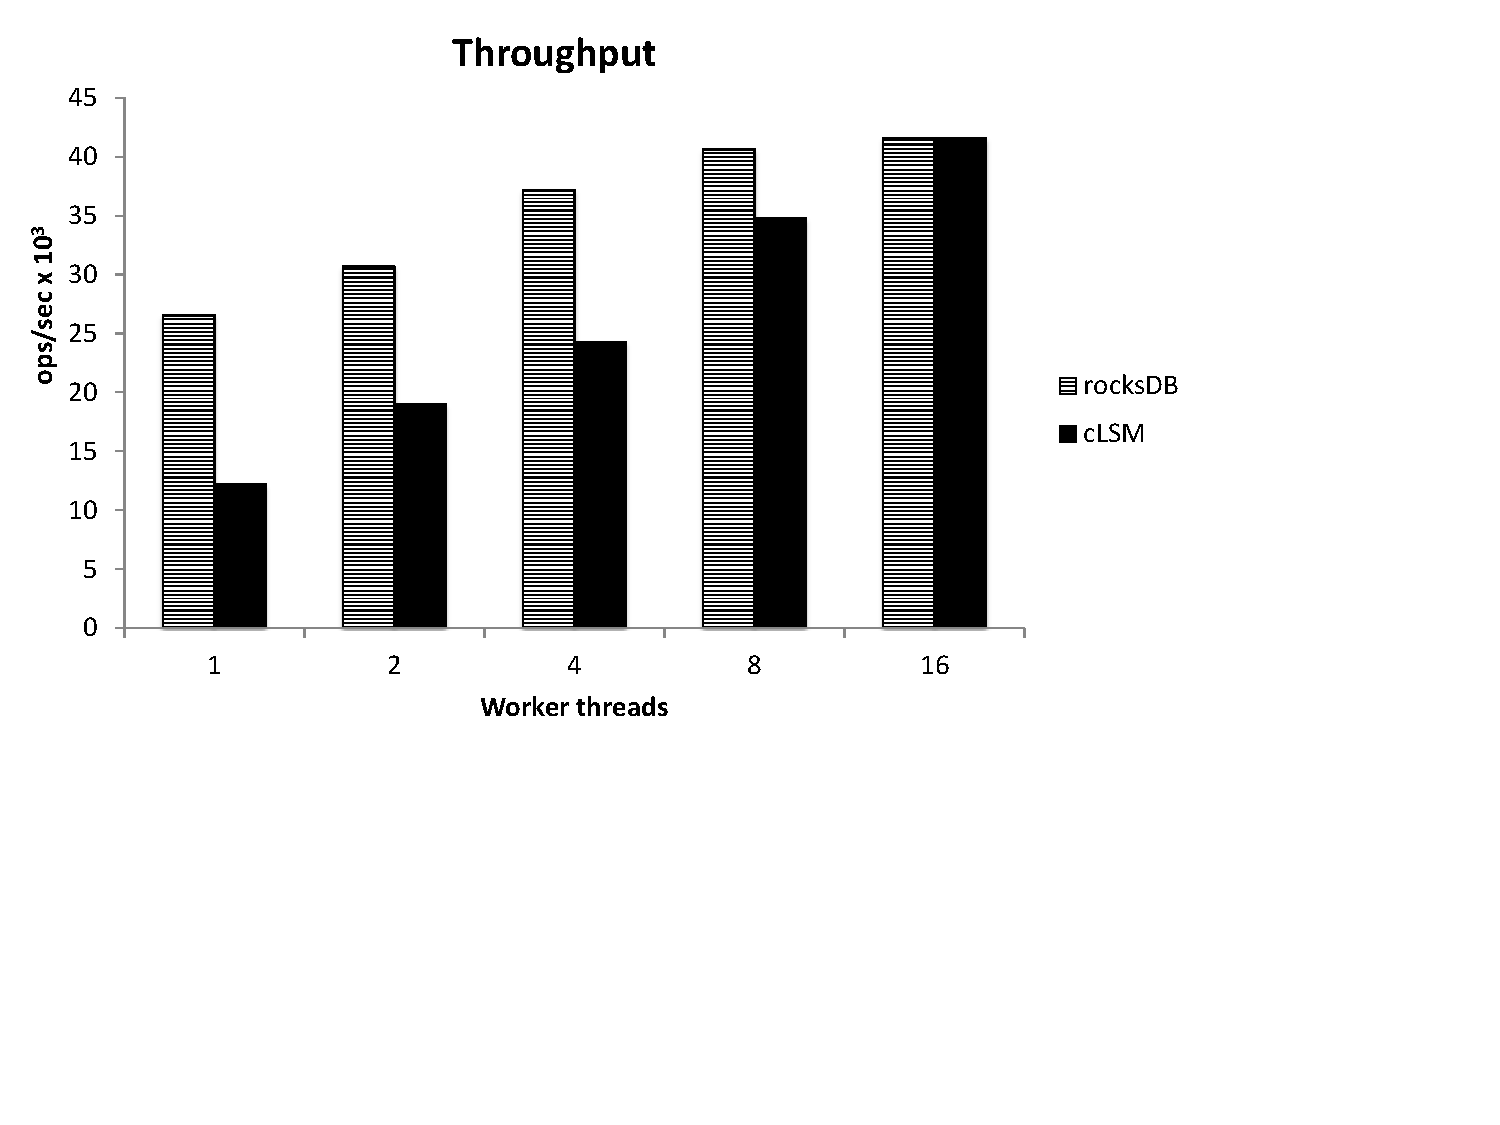
\includegraphics[width=0.45\textwidth,clip, trim =0 180 150 0]{Figures/HeavyCompactions.pdf}}
}
\caption{\bf{Workload with heavy disk-compaction.}}
\label{fig:HeavyCompactions}
\end{figure}
%}




